%TCIDATA{LaTeXparent=0,0,relatorio.tex}
\ifx\compilewholereport\undefined
	\documentclass[11pt,a4paper,oneside]{book}
	
	% Escolher um dos seguintes formatos:
	\usepackage{ft2unb} % segue padrão de fontes do Latex
	
	% Pacotes
	\usepackage{graphicx}
	\usepackage{amsfonts}
	\usepackage{amsmath}
	\usepackage{amssymb}
	\usepackage[thmmarks,amsmath]{ntheorem}
	\usepackage{boxedminipage}
	\usepackage{theorem}
	\usepackage{fancybox}
	\usepackage{fancyhdr}
	\usepackage{url}
	\usepackage{afterpage}
	\usepackage{color}
	\usepackage{colortbl}
	\usepackage{rotating}
	\usepackage{makeidx}
	\usepackage{indentfirst}
	\usepackage{bibentry}
	\usepackage{subcaption}
	\usepackage{todonotes}
	\presetkeys{todonotes}{inline}{}
	
	\begin{document}
	\frontmatter
	\listoftodos
	\mainmatter
	
	%%%%%%%%%%%%%%%%%%%%%%%%%%%%
	%%%%%%%% Apagar coisas acima
	%%%%%%%%%%%%%%%%%%%%%%%%%%%%
\fi

\chapter{Introdu\c{c}\~ao}\label{CapIntro}

\resumodocapitulo{Este cap\'itulo contextualiza o tema apresentado, apresentando a motivação histórica para o desenvolvimento do mesmo.}

\section{Introdu\c{c}\~ao} 
O mundo atual \'e controlado quase que completamente por sistemas digitais.
As informa\c{c}\~oes obtidas pelos sensores s\~ao digitalizadas antes de serem tratadas.
Tal processo de digitaliza\c{c}\~ao \'e importante, visto que elimina os ru\'idos intr\'insecos ao processamento anal\'ogico \cite{chen2004electrical}.

O primeiro computador de computa\c{c}\~ao gen\'erica surgiu por volta da d\'ecada de 40.
Sua inven\c{c}\~ao iniciou a terceira revolu\c{c}\~ao industrial, conhecida como revolu\c{c}\~ao da informa\c{c}\~ao ou revolu\c{c}\~ao t\'ecnico-cient\'ifica-informacional \cite{patterson2005coa}.
Os computadores dessa \'epoca liam e executavam instru\c{c}\~oes de forma linear, em um modelo conhecido como sequencial ou temporal. 

Nos anos que se seguiram, a substituição das válvulas por transistores de sil\'icio ajudaram a reduzir o tamanho dos computadores de metros a cent\'imetros quadrados.
Tal mudan\c{c}a permitiu um aumento na popularidade destes dispositivos para o uso pessoal, efeito que impulsionou a ind\'ustria de produ\c{c}\~ao de processadores \cite{Hennessy2011}.
As empresas da \'epoca come\c{c}aram ent\~ao a guerra de miniaturiza\c{c}\~oes de transistores, marcada pelo c\'elebre artigo de Gordon E. Moore, cofundador da Intel, que dizia que o n\'umero de transistores dentro de um processador duplicaria aproximadamente a cada 2 anos \cite{Moore1965}.
A partir de 1970, a lei foi adaptada para a duplica\c{c}\~ao a cada 18 meses.

\begin{figure}[h]
	\centering
	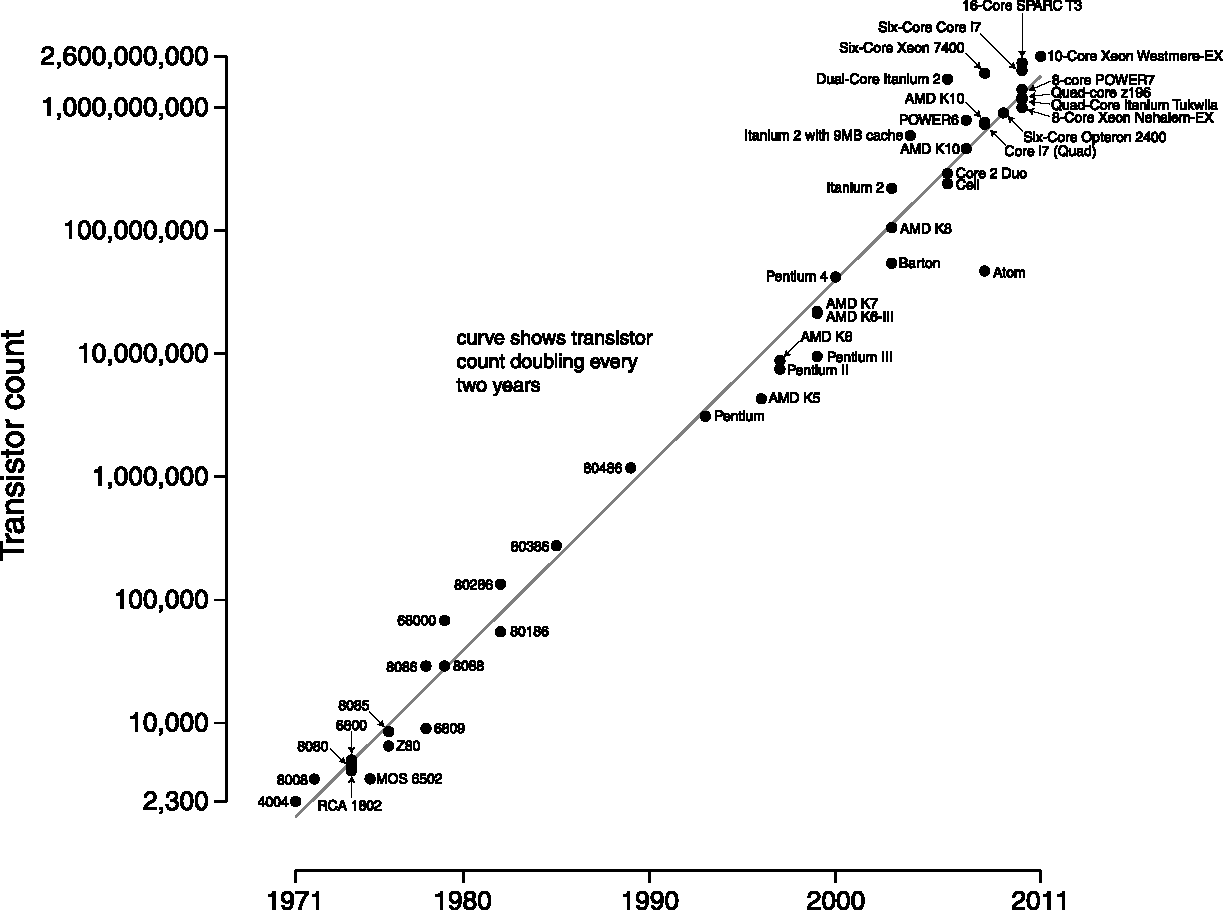
\includegraphics[width=0.7\textwidth]{fig/c1_introducao/moores_law.pdf}
	\caption{Visualização da Lei de Moore. Eixos em escala logarítmica. Gráficos extraidos do Wikipedia sob licença \textit{Creative Commons}.}
	\label{fig:moores_law}
\end{figure}

Com a integra\c{c}\~ao de mais componentes dentro do processador, conjuntos de instru\c{c}\~oes cada vez mais complexas foram desenvolvidas.
Estas intru\c{c}\~oes surgiram para acelerar a computa\c{c}\~ao de fun\c{c}\~oes de n\'iveis mais altos.
A integra\c{c}\~ao tamb\'em reduziu a pot\^encia dissipada por transistor, permitindo que as frequ\^encias de opera\c{c}\~ao dos computadores fosse aumentada \cite{Hennessy2011}.

Com o aumento da complexidade das instruções, passou-se a adotar duas nomenclaturas diferentes para processadores: \textit{Reduced Instruction Set Computer} (RISC) e \textit{Complex Instruction Set Computer} (CISC) \cite{Fedeli2003}.
A arquitetura RISC possui um conjunto pequeno e muito otimizado de funções, comandos exclusivos para acesso a memória (arquitetura \textit{load/store}) e uma média de uma instrução completada por ciclo, quando desconsidera-se as instruções de acesso a memória.
A arquitetura CISC possui várias funções para tarefas mais específicas, que por vezes demandam vários ciclos de relógio, e funções que realizam operações com informações lendo e/ou salvando direto na/para a memória.
Ambas arquiteturas são muito utilizadas nos dias de hoje, sendo as RISC mais comum em dispositivos com restrições de consumo de energia e as CISC mais comuns em dispositivos de computação mais genérica.

\todo{Falar mais sobre RISC e CISC (Patterson \url{file:///E:/resources/Chapters/CD2.20-P374493.pdf}.}

\begin{figure}[h]
\centering
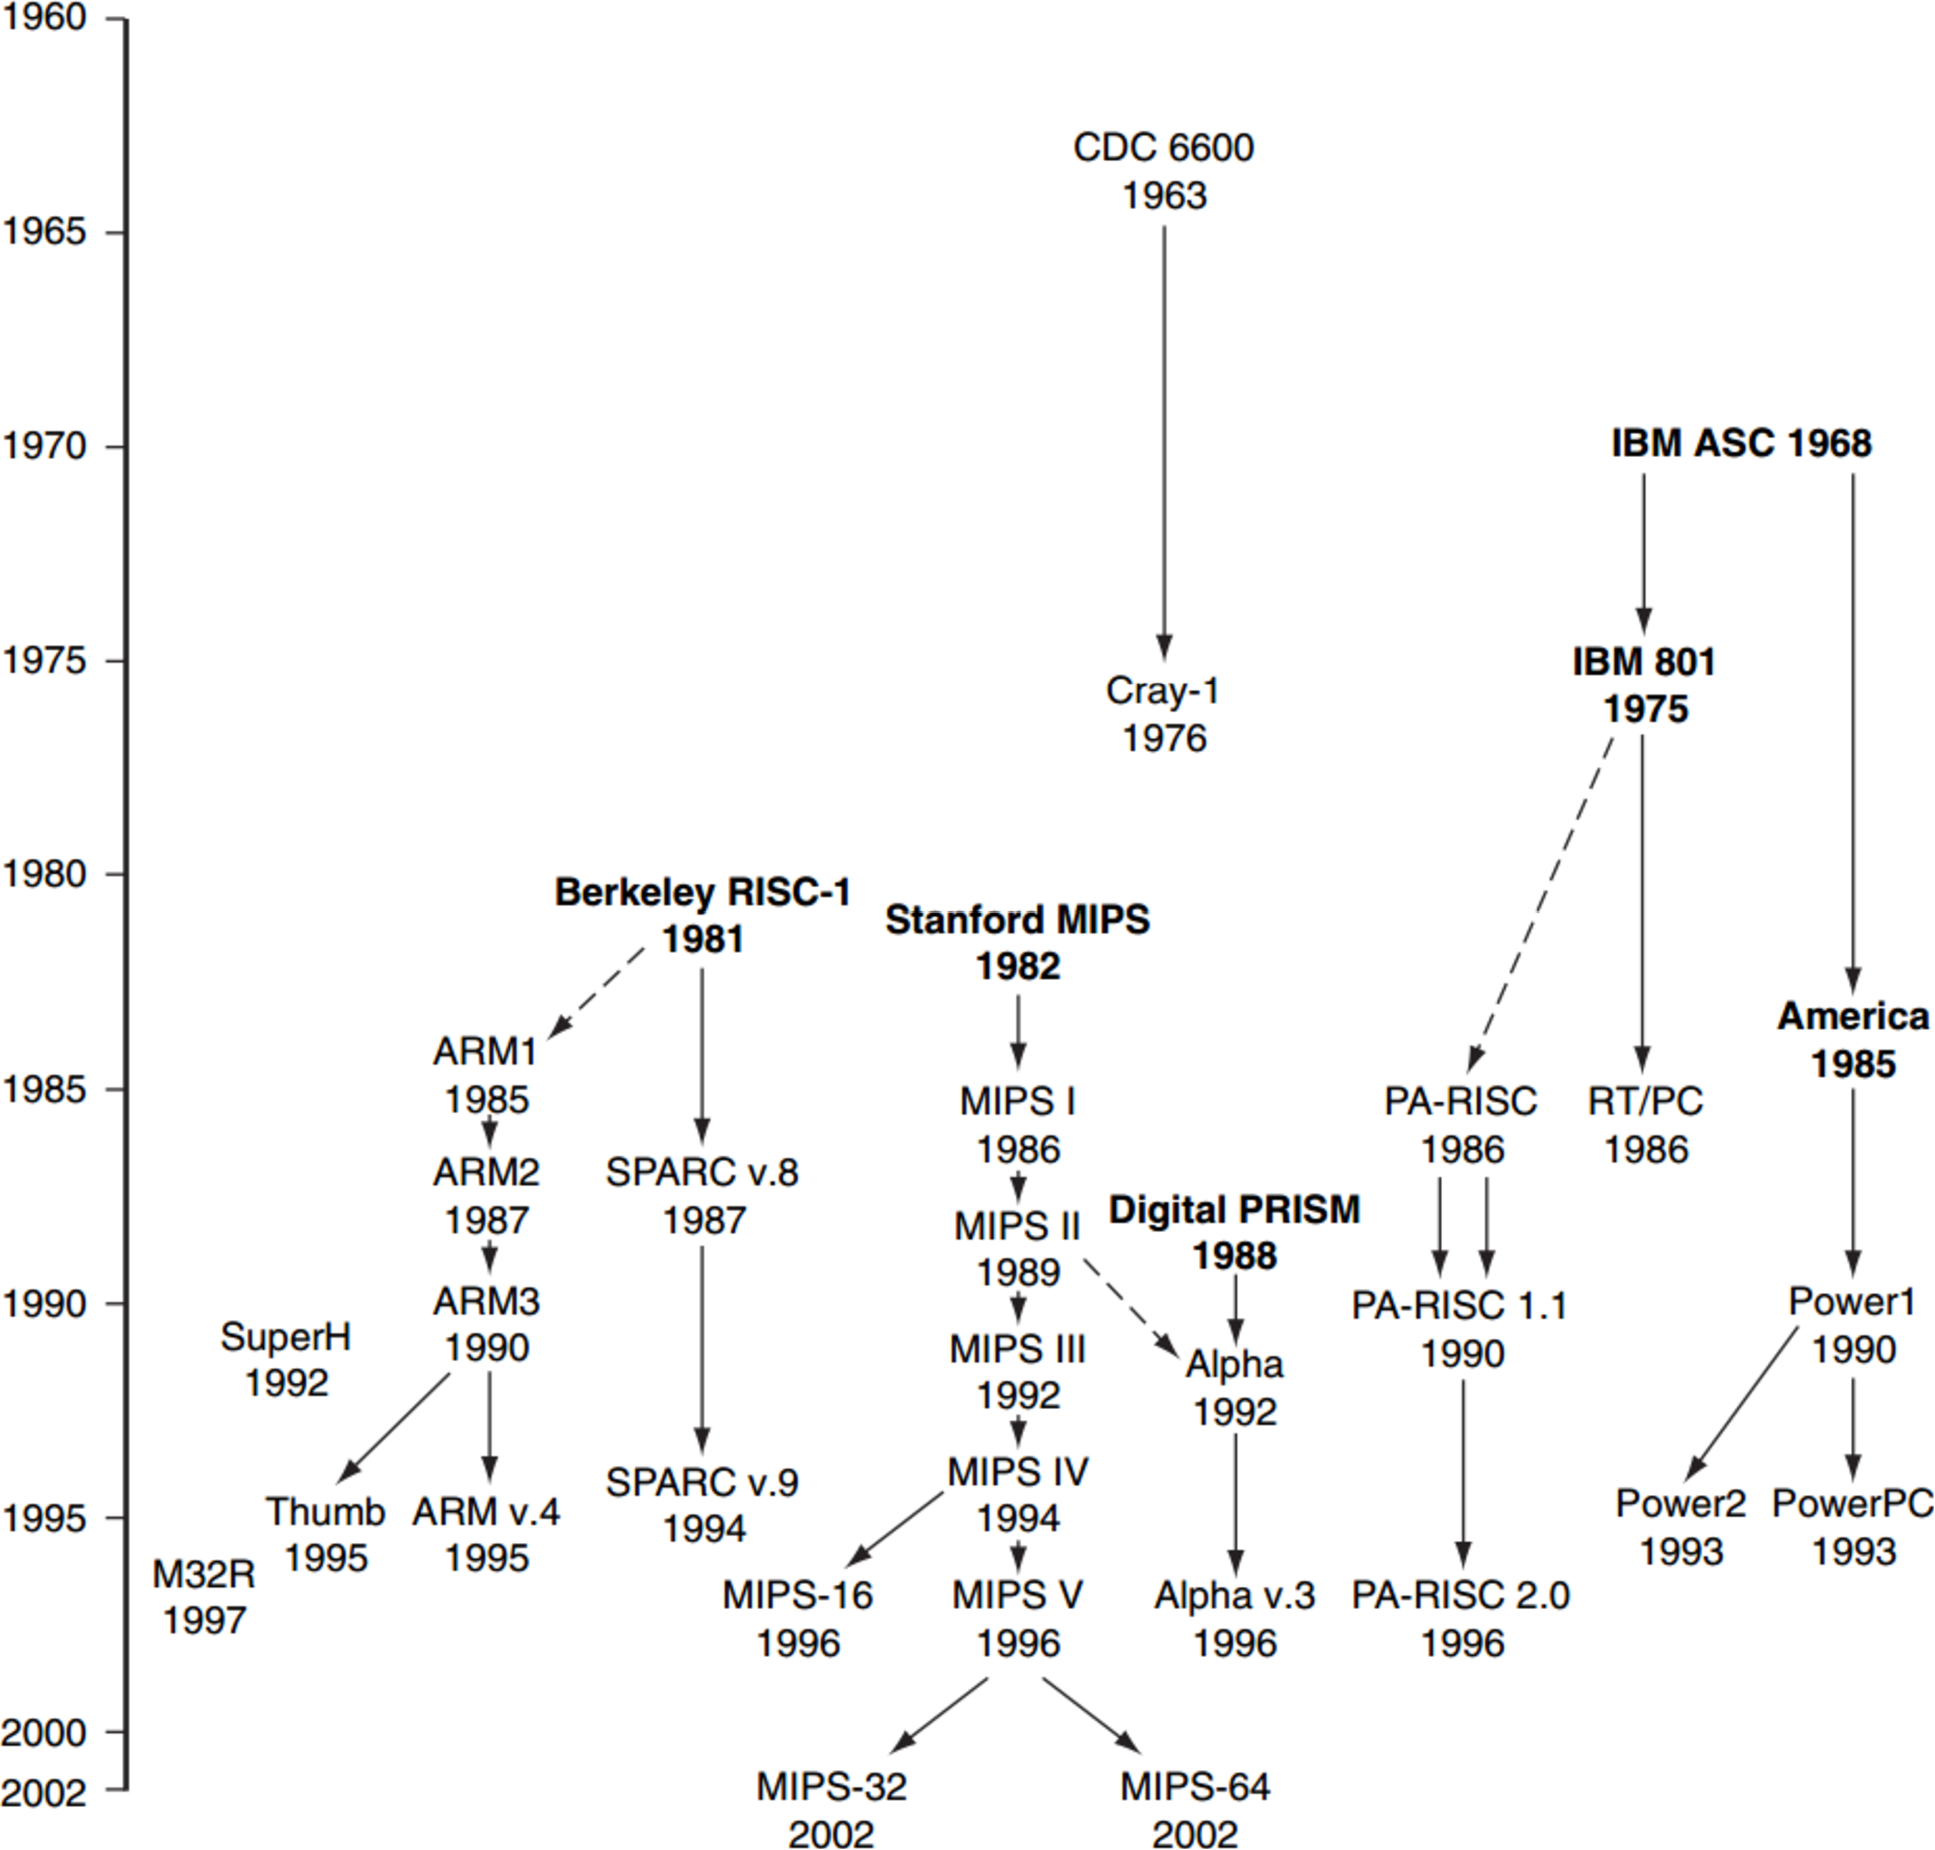
\includegraphics[width=0.7\textwidth]{fig/c1_introducao/history_risc.pdf}
\caption{Linha do tempo das arquiteturas RISC, extraido de \cite{Hennessy2011}. Em negrito estão as iniciativas de pesquisa, em contraste às comerciais.}
\label{fig:history_risc}
\end{figure}

Por volta dos anos 2000, a pot\^encia dissipada em cada transistor, proporcional a frequência de opera\c{c}\~ao, havia atingido o limite suportado pelo microprocessador.
Por causa disso, o crescimento desenfreado da frequ\^encia teve que ser repensado.
Come\c{c}ou-se ent\~ao o desenvolvimento de microprocessadores \textit{multicore}, que aumentam a vaz\~ao de instru\c{c}\~oes (\textit{throughtput}) sem modificar o tempo de resposta, que corresponde ao tempo de processamento médio de uma instrução.
Em meados de 2006, todas as grandes companhias j\'a possuiam produtos com esta arquitetura \cite{Hennessy2011}.

Os microprocessadores com v\'arios n\'ucleos (\textit{multicore}) abriram espa\c{c}o para a chegada de processadores com muitos n\'ucleos (\textit{manycore}).
Estes microprocessadores s\~ao projetados para placas gr\'aficas e, apesar de possuirem centenas de n\'ucleos, estes núcleos s\~ao simplificados \cite{Vajda2011}.
Em geral, eles são capazes de realizar apenas algumas poucas operações, mas abrem caminho para paradigmas de programação que transformem a computação concorrente em computação paralela \cite{Harel2004}.

Mesmo trabalhando com um ou v\'arios n\'ucleos de processamento, o modelo de computa\c{c}\~ao atual ainda \'e dito temporal ou sequencial uma vez que blocos de instru\c{c}\~oes s\~ao executados em seu devido instante de tempo de forma sequencial, conceito destacado pela atomicidade estudada em programa\c{c}\~ao paralela \cite{williams2012c++}.

Do ponto de vista da programa\c{c}\~ao, os primeiros computadores apresentavam programas que n\~ao podiam ser alterados.
Parte desta limita\c{c}\~ao era justificada pela programa\c{c}\~ao utilizando-se cart\~oes, mas nas primeiras gera\c{c}\~oes de computadores com mem\'orias eletr\^onicas o mesmo sistema foi utilizado.

A arquitetura de von Neumann, utilizada na primeira gera\c{c}\~ao de computadores eletr\^onicos, era cons\-ti\-tu\'i\-­da de uma \'unica unidade de mem\'oria, uma unidade de processamento e um canal de comunica\c{c}\~ao.
Esta arquitetura possui tanto uma vantagem tremenda, a capacidade de modifica\c{c}\~ao de programas em tempo de execu\c{c}\~ao, quanto uma falha crucial, conhecida por gargalo de von Neumann.
A vantagem aparece uma vez que, como n\~ao h\'a distin\c{c}\~ao entre mem\'oria de programa e dados, uma instru\c{c}\~ao pode sobrescrever um endere\c{c}o de mem\'oria marcado como programa.
O problema diz respeito \`as restri\c{c}\~oes impostas pelo canal de comunica\c{c}\~ao, que permitia que apenas uma palavra, seja de programa ou de dados, fosse mandada para a unidade de processamento e de volta \cite{Backus1978}.
Este problema se agrava a medida que o processador fica mais r\'apido que a mem\'oria, uma vez que o tempo de espera, em ciclos de rel\'ogios, para a obten\c{c}\~ao da informa\c{c}\~ao aumenta.
Para solucionar o problema do gargalo de von Neumann, a arquitetura Harvard foi proposta.

A arquitetura Harvard original propunha que a mem\'oria de programa e a mem\'oria de dados fossem fisicamente separadas e possuissem cada uma seu pr\'oprio canal de comunica\c{c}\~ao com o processador.
Essa modifica\c{c}\~ao acelera a execu\c{c}\~ao de certos programas, visto que programa e dados podem ser carregados das suas respectivas mem\'orias simultaneamente.
Uma pequena altera\c{c}\~ao na arquitetura Harvard, conhecida de arquitetura Harvard modificada, permitia que mais de um canal de comunica\c{c}\~ao ligasse a uma mem\'oria tanto de programa quanto de dados.
Essas informa\c{c}\~oes eram divididas em mem\'orias tempor\'arias (\textit{cache}) espec\'i­ficas para o programa e para dados, formando assim uma arquitetura Harvard original.
Essa modifica\c{c}\~ao combina os benef\'i­cios da arquitetura de von Neumann, ou seja, a modifica\c{c}\~ao de programas em tempo de execu\c{c}\~ao, e da arquitetura Harvard original, ou seja, o tempo de acesso reduzido.

Atualmente, nossos modernos computadores multiprocessados utilizam a arquitetura Harvard modificada com diversos n\'i­veis de mem\'oria \textit{cache} \cite{Hennessy2011}, sejam eles dedicados ou compartilhados entre os v\'arios processadores.
A sua capacidade de processamento atinge n\'i­veis extraordin\'arios, ultrapassando 20 GFlops em computadores comuns \cite{MaxxPI2013} e 54 PFlops em supercomputadores \cite{Top5002013}.
Apesar disso, a arquitetura Harvard original ainda \'e muito usada em microcontroladores e processadores digitais de sinal (\textit{Digital Signal Processors} ou DSPs).

\todo{Comentar benchmarking e como eles perdem um pouco do sentido com a configuração de hardware (Patterson \url{file:///E:/resources/Chapters/CD1.10-P374493.pdf}).}

\subsection{Computa\c{c}\~ao Reconfigur\'avel}
\label{ss:computacao_reconfiguravel}

A computa\c{c}\~ao reconfigur\'avel foi proposta por volta de 1960 por Gerald Estrin para resolver problemas que n\~ao podiam ser resolvidos pela computa\c{c}\~ao da \'epoca \cite{Estrin2002}.
Estrin prop\^os um microprocessador composto de uma parte fixa e uma parte vari\'avel, onde a parte vari\'avel seria usada para programar funcionamentos espec\'i­ficos para serem usados em determinados per\'i­odos de tempo.
A id\'eia de Estrin foi deixada de lado \`a medida que os microprocessadores e \textit{Application-Specific Integrated Circuits} (ASICs) se mostraram aptos a resolver os problemas da \'epoca.
Por volta da d\'ecada de 1990, por\'em, o primeiro microprocessador h\'i­brido comercial foi desenvolvido \cite{Estrin2002}, trazendo novamente esta tecnologia \`a tona.

A tecnologia inventada por Estrin, tamb\'em conhecido como estrutura \textit{Fixed Plus Variable} (F+V), trouxe \`a tona um novo paradigma de processamento de dados \cite{Hartenstein2001}.
O motivo para tal \'e o fato de que a intera\c{c}\~ao entre as unidades de processamento e os dados mudou completamente.
O que antes se conhecia por modelo temporal de computa\c{c}\~ao foi deixado de lado para, nesta nova arquitetura, se tornar um modelo espacial.
Em outras palavras, os dados n\~ao eram direcionados um a um para uma unidade central de processamento, mas processados continuamente em um sistema distribu\'i­do no espa\c{c}o \cite{vassiliadis2007fine}.
Tal sistema distribu\'i­do \'e composto de c\'elulas l\'ogicas e suas conex\~oes, ambas reprogram\'aveis, ajudando a se alcan\c{c}ar uma efici\^encia similar a presente em ASICs e flexivel como a computa\c{c}\~ao gen\'erica.

\begin{figure}[h]
\centering
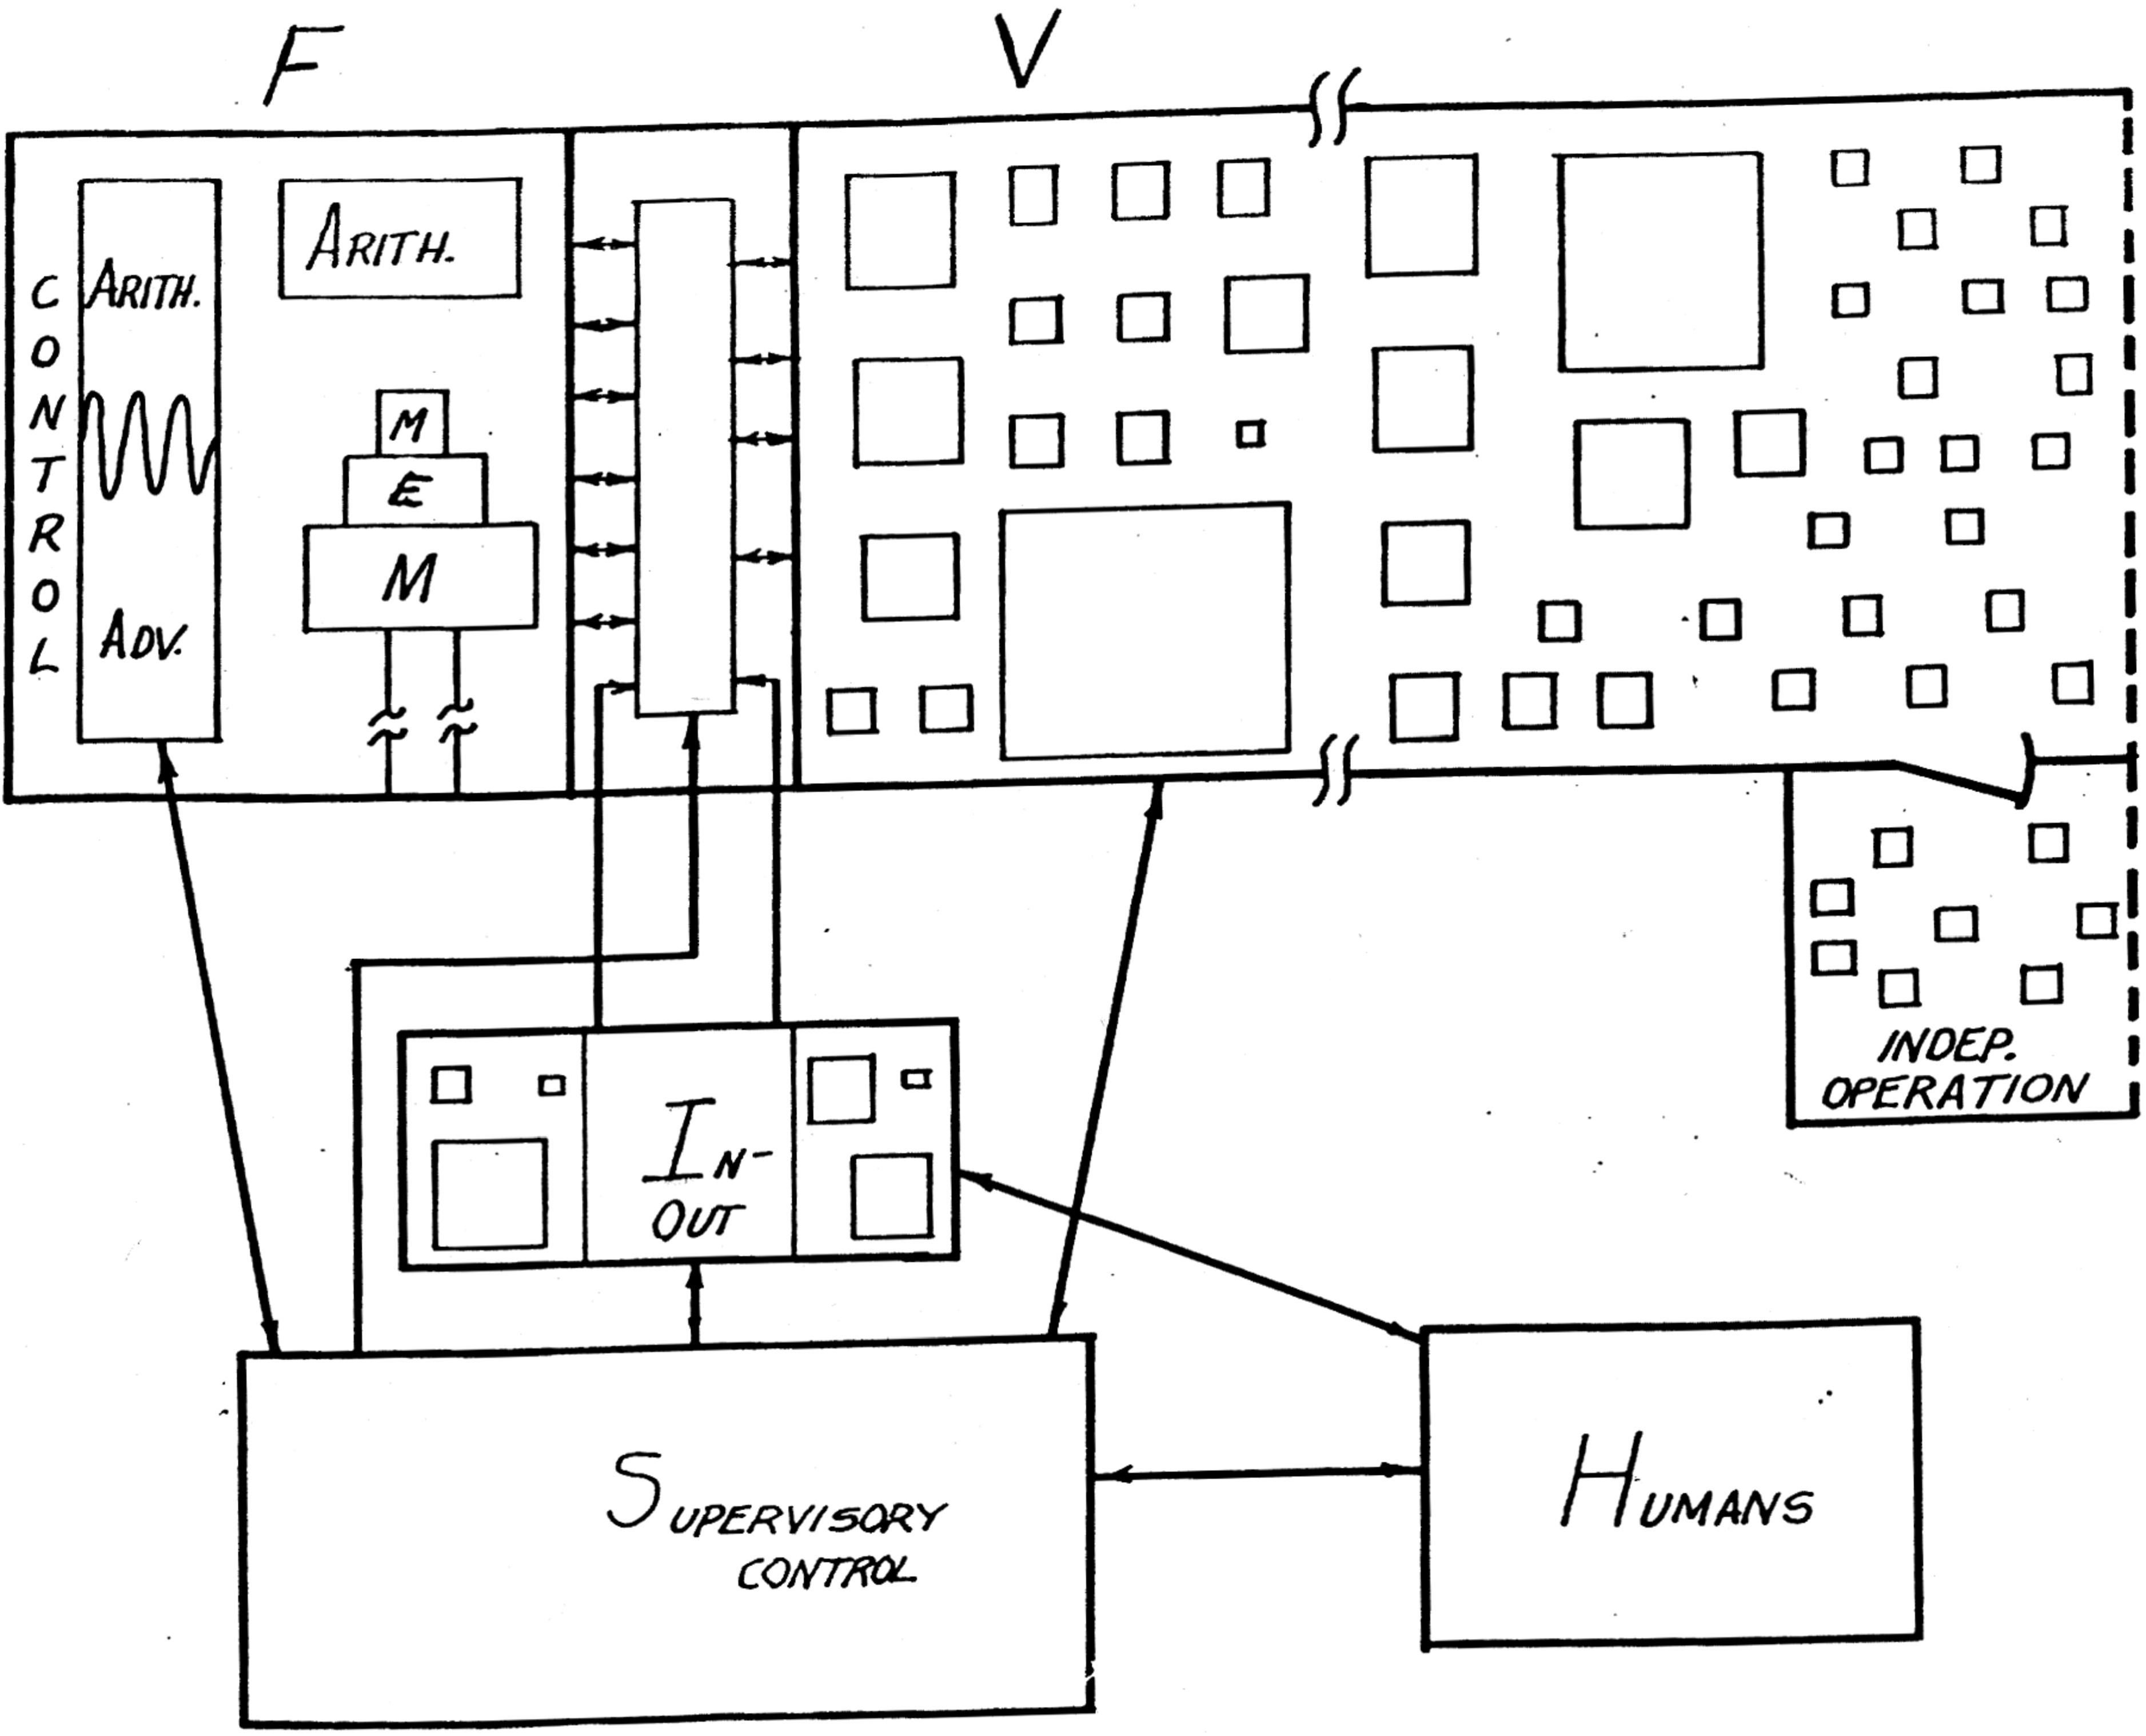
\includegraphics[width=0.7\textwidth]{fig/c1_introducao/model_f+v.pdf}
\caption{Esquem\'atico com o F+V, extraido de \cite{Estrin2002}.}
\label{fig:model_f+v}
\end{figure}

Ao contr\'ario da estrutura F+V proposta por Estrin, a maioria dos sistemas reconfigur\'aveis atuais possuem apenas a parte reconfigur\'avel.
Apesar de sistemas reconfigur\'aveis de alta performance possuirem componentes fixos como processadores e unidades de processamento gr\'aficos (GPUs) \cite{El-Ghazawi2008}, a sua aus\^encia reduz o custo de projeto e a flexibilidade do projeto final.

Os sistemas reconfigur\'aveis atuais utilizam de tr\^es meios principais de programa\c{c}\~ao: \textit{Static Random-Access Memory} (SRAM), \textit{Antifuse} e mem\'orias n\~ao-vol\'ateis.
Usando SRAM, o resultado da s\'i­ntese
%, processo comentado na se\c{c}\~ao \ref{sss:sintese},
 \'e armazenado nas c\'elulas desta mem\'oria e controlam o estado dos transistores das c\'elulas l\'ogicas.
No caso de c\'elulas compostas de tabelas de busca (\textit{look-up tables} ou LUTs), a SRAM armazena os dados dessas c\'elulas.
Outra segunda tecnologia de programa\c{c}\~ao, o \textit{antifuse}, faz uso de uma conex\~ao com imped\^ancia vari\'avel, onde atrav\'es do uso de altas voltagens pode-se modificar a resist\^encia de uma via.
Esse processo de programa\c{c}\~ao \'e irrevers\'i­vel.
As mem\'orias n\~ao vol\'ateis, como EPROM, EEPROM e FLASH, usam transistores especiais com uma ponte flutuante.
Quando a ponte possui carga, o transistor pode ser controlado pela ponte de sele\c{c}\~ao, que permanece carregada at\'e quando desligada.
Estas t\'ecnicas permitem a resist\^encia da \textit{antifuse} e a reprogramabilidade da SRAM, sendo apenas mais complexa e demorada para ser programada \cite{vassiliadis2007fine}.

As interconex\~oes entre c\'elulas l\'ogicas, que logicamente influenciam diretamente as c\'elulas em si, podem ser de cinco tipos: ilha, linha, mar-de-portas, hier\'arquico e estruturas unidimensionais \cite{vassiliadis2007fine}.
A arquitetura do tipo ilha consiste em c\'elulas l\'ogicas conectadas umas as outras atrav\'es de caixas de conex\~oes e de roteamento.
Nesta arquitetura, a c\'elula l\'ogica est\'a cercada por trilhas de conex\~oes, o que explica o nome.
A arquitetura do tipo linha consiste em v\'arias linhas divididas em quantidades variadas de segmentos.
As conex\~oes s\~ao ent\~ao realizadas usando-se linhas verticais atrav\'es de blocos l\'ogicos especiais.
A arquitetura do tipo mar-de-portas consiste de blocos l\'ogicos que cobrem todo o espa\c{c}o do dispositivo e s\~ao conectados aos seus vizinhos diretos.
Em geral este tipo de conex\~ao \'e mais r\'apido.
A arquitetura do tipo hier\'arquico agrupa as c\'elulas l\'ogicas em \textit{clusters}, e agrupa estes em \textit{clusters} de mais alto n\'i­vel, formando de fato um sistema hier\'arquico.
O \'ultimo tipo de arquitetura, unidimensional, surge como uma tentativa de simplificar o roteamento complexo dos sistema bidimensionais apresentados anteriormente.
Nele, restri\c{c}\~oes de aloca\c{c}\~ao e roteamento s\~ao impostas para reduzir o n\'umero de possibilidades.
O problema deste tipo de arquitetura \'e que se n\~ao houverem recursos de roteamento suficientes, o roteamento fica mais complexo que nas arquiteturas bidimensionais.

As arquiteturas reconfigur\'aveis podem ser classificada em tr\^es tipos segundo a granularidade.
A granularidade diz respeito a quantidade de informa\c{c}\~ao m\'i­nima que pode ser passada de uma c\'elula l\'ogica para outra.
Ela separa as arquiteturas reconfigur\'aveis em tr\^es categorias: granularidade fina, grossa e h\'i­brida.
Nas arquiteturas com granularidade fina, como os \textit{Field-Programmable Gate Arrays}, um \'unico \textit{bit} pode ser transferido de uma c\'elula a outra, permitindo assim um maior controle sobre os dados.
Nas arquiteturas com granularidade grossa, os \textit{bits} s\~ao agrupados em palavras de tamanhos fixos, reduzindo assim o espa\c{c}o gasto com roteamento e melhorando a roteabilidade \cite{Hartenstein2001}.
No \'ultimo tipo de arquiteturas, a h\'i­brida, parte das conex\~oes s\~ao grossas e partes s\~ao finas, combinando os benef\'i­cios das duas classes.

As formas mais comuns de dispositivos reconfigur\'aveis s\~ao o \textit{Programmable Array Logic} (PAL), o \textit{Complex Programmable Logic Device} (CPLD), o \textit{Field-Programmable Gate Array} e o \textit{Reconfigurable Datapath Array} (rDPA).
Cada um possui suas vantagens e desvantagens segundo a forma de implementa\c{c}\~ao, comentadas a seguir.

\begin{figure}[h]
\centering
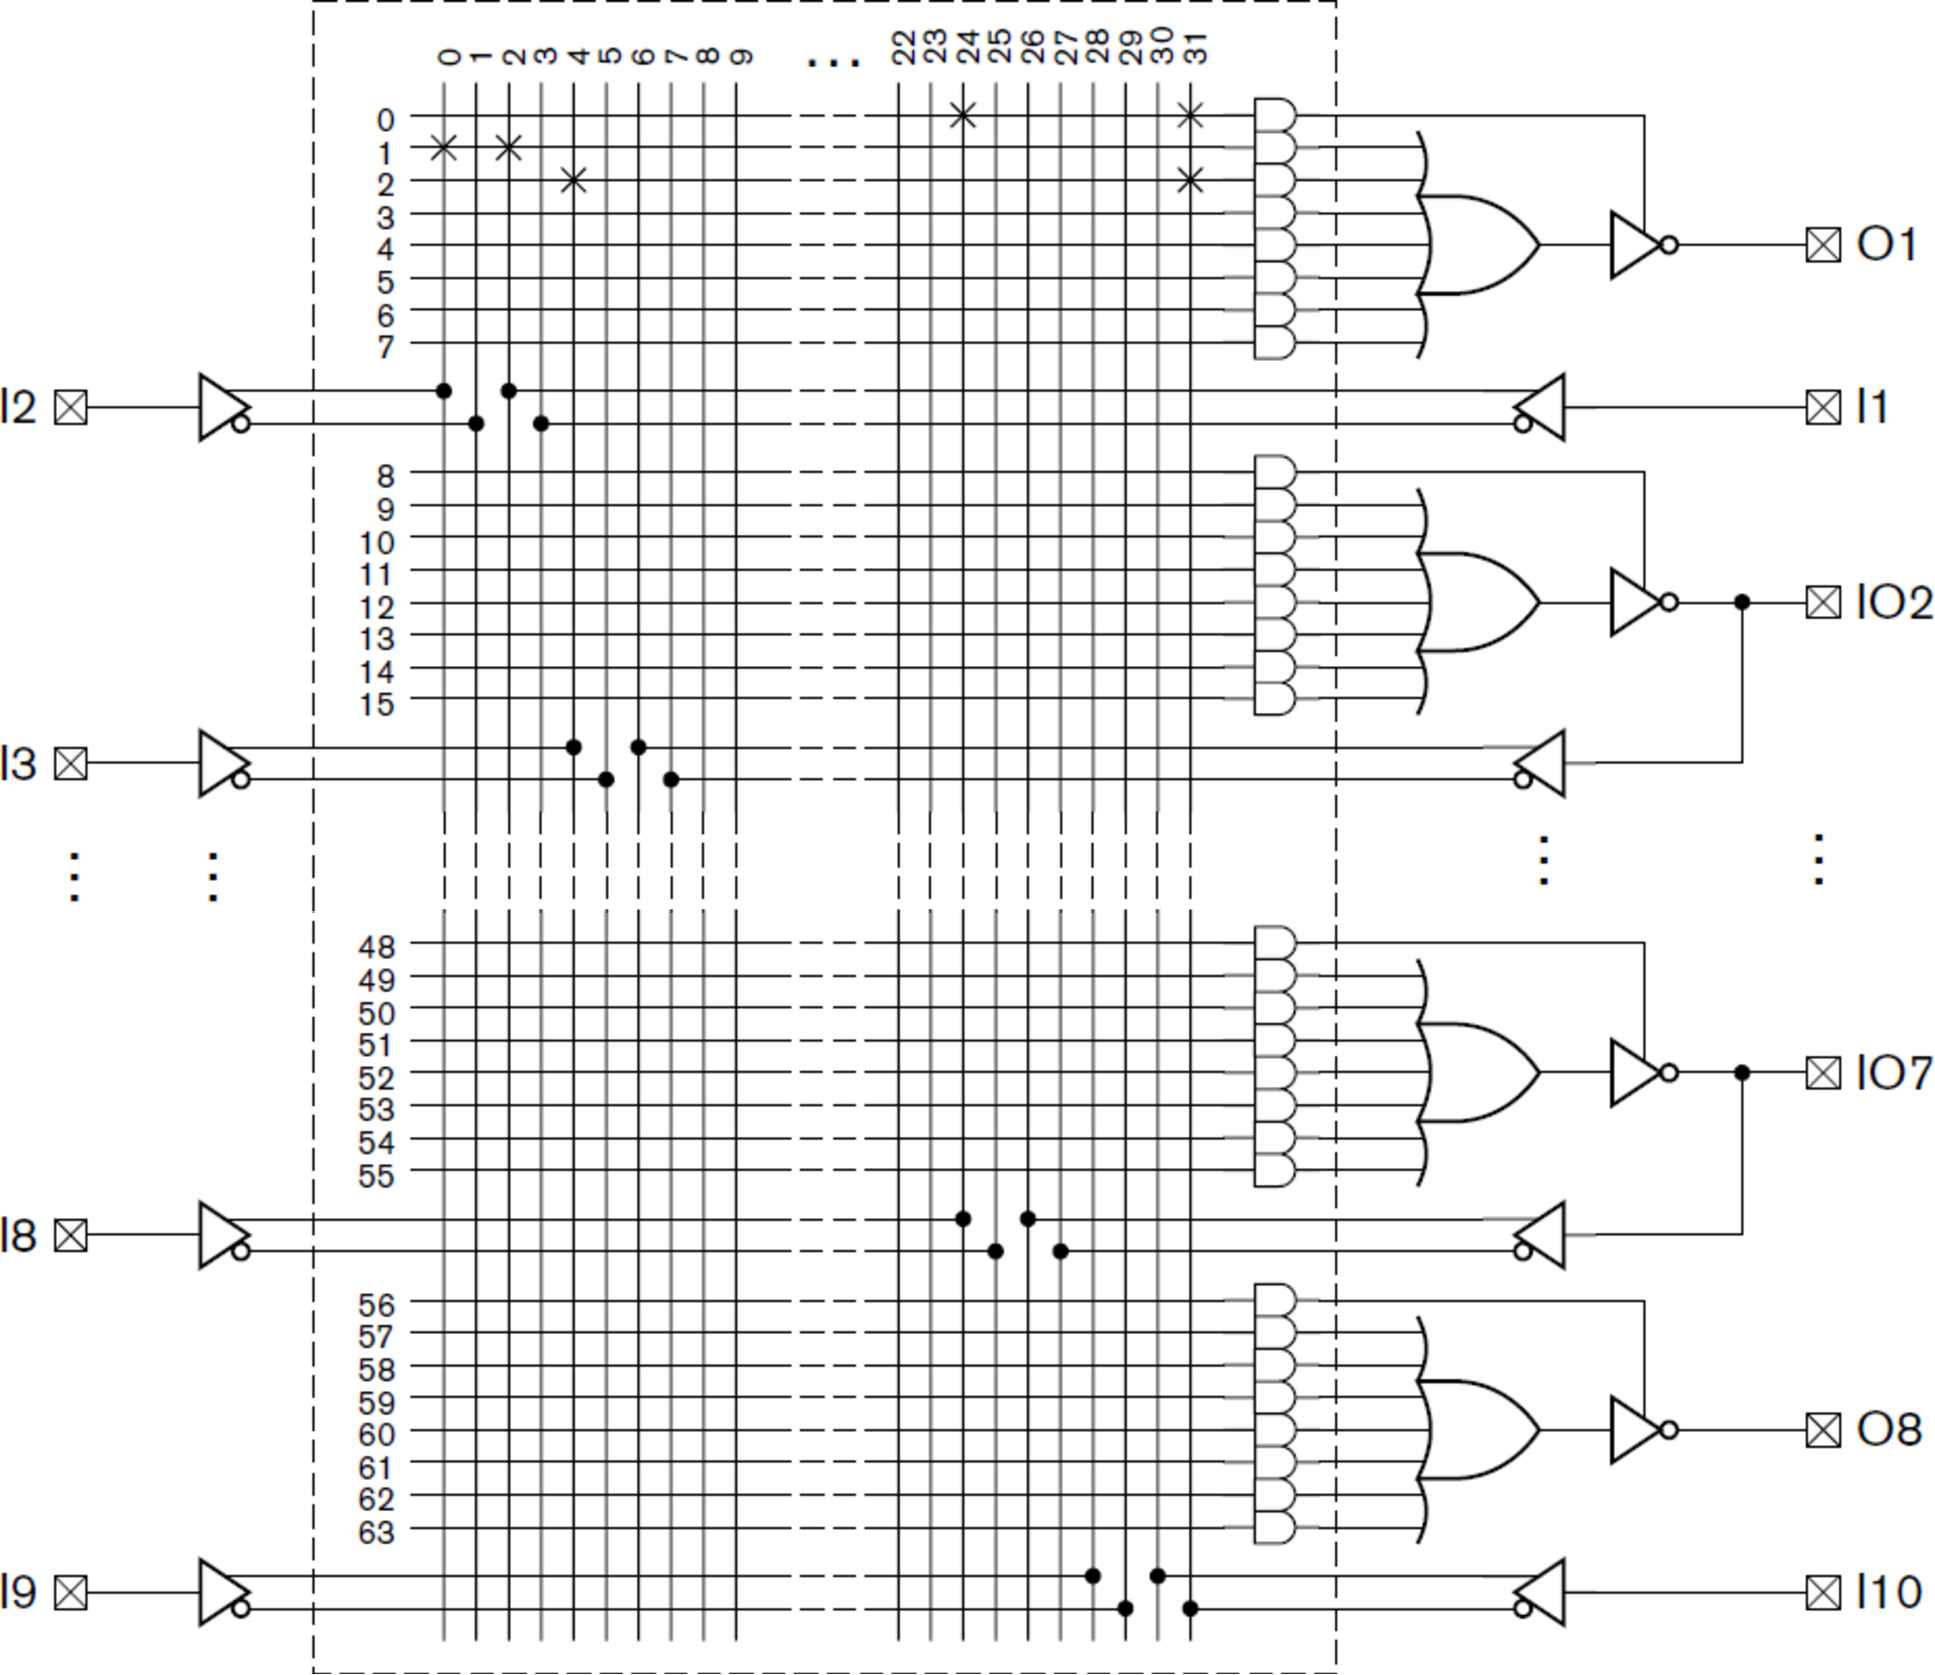
\includegraphics[width=0.7\textwidth]{fig/c1_introducao/model_pal.pdf}
\caption{Circuito interno de um dispositivo do tipo PAL, extraido de \cite{Ashenden2008}.}
\label{fig:pal}
\end{figure}

\paragraph{\textit{Programmable Array Logic}}
Os \textit{Programmable Array Logics} (PALs) foram os primeiros dispositivos program\'aveis, desenvolvidos por volta de 1970.
Os PALs podem ser configurados para desempenhar diversas fun\c{c}\~oes l\'ogicas com possibilidade de cascateamento.
Alguns tipos especiais de PALs tamb\'em cont\'em registradores, permitindo a programa\c{c}\~ao de circuitos sequenciais simples.
Outra caracter\'i­stica dos PALs que permitiam a constru\c{c}\~ao de circuitos l\'ogicas um pouco mais complexas era a realimenta\c{c}\~ao, como pode ser visto na figura \ref{fig:pal}.
Eles podem ser programados usando uma linguagem de descri\c{c}\~ao de \textit{hardware} com informa\c{c}\~oes na forma de express\~oes booleanas.
Eles por\'em se tornaram obsoletos com a chegada dos \textit{Generic Array Logics} (GALs) e \textit{Complex Programmable Logic Devices} (CPLDs).
Eles eram produzidos principalmente pela Data I/O Corporation.

Os PALs surgiram para substituir a l\'ogica TTL, usada em granda escala na prototipagem e em dispositivos pequenos.
Em geral, mesmo que para projetos com apenas alguns elementos de l\'ogica TTL, o uso de PALs possu\'i­a um custo e confiabilidade maiores que na combina\c{c}\~ao de v\'arios \textit{chips} diferentes.
Sua programa\c{c}\~ao \'e feita atrav\'es de conex\~oes compostas por pequenos fus\'i­veis, que s\~ao queimados quando a conex\~ao n\~ao \'e necess\'aria.

\begin{figure}[h]
\centering
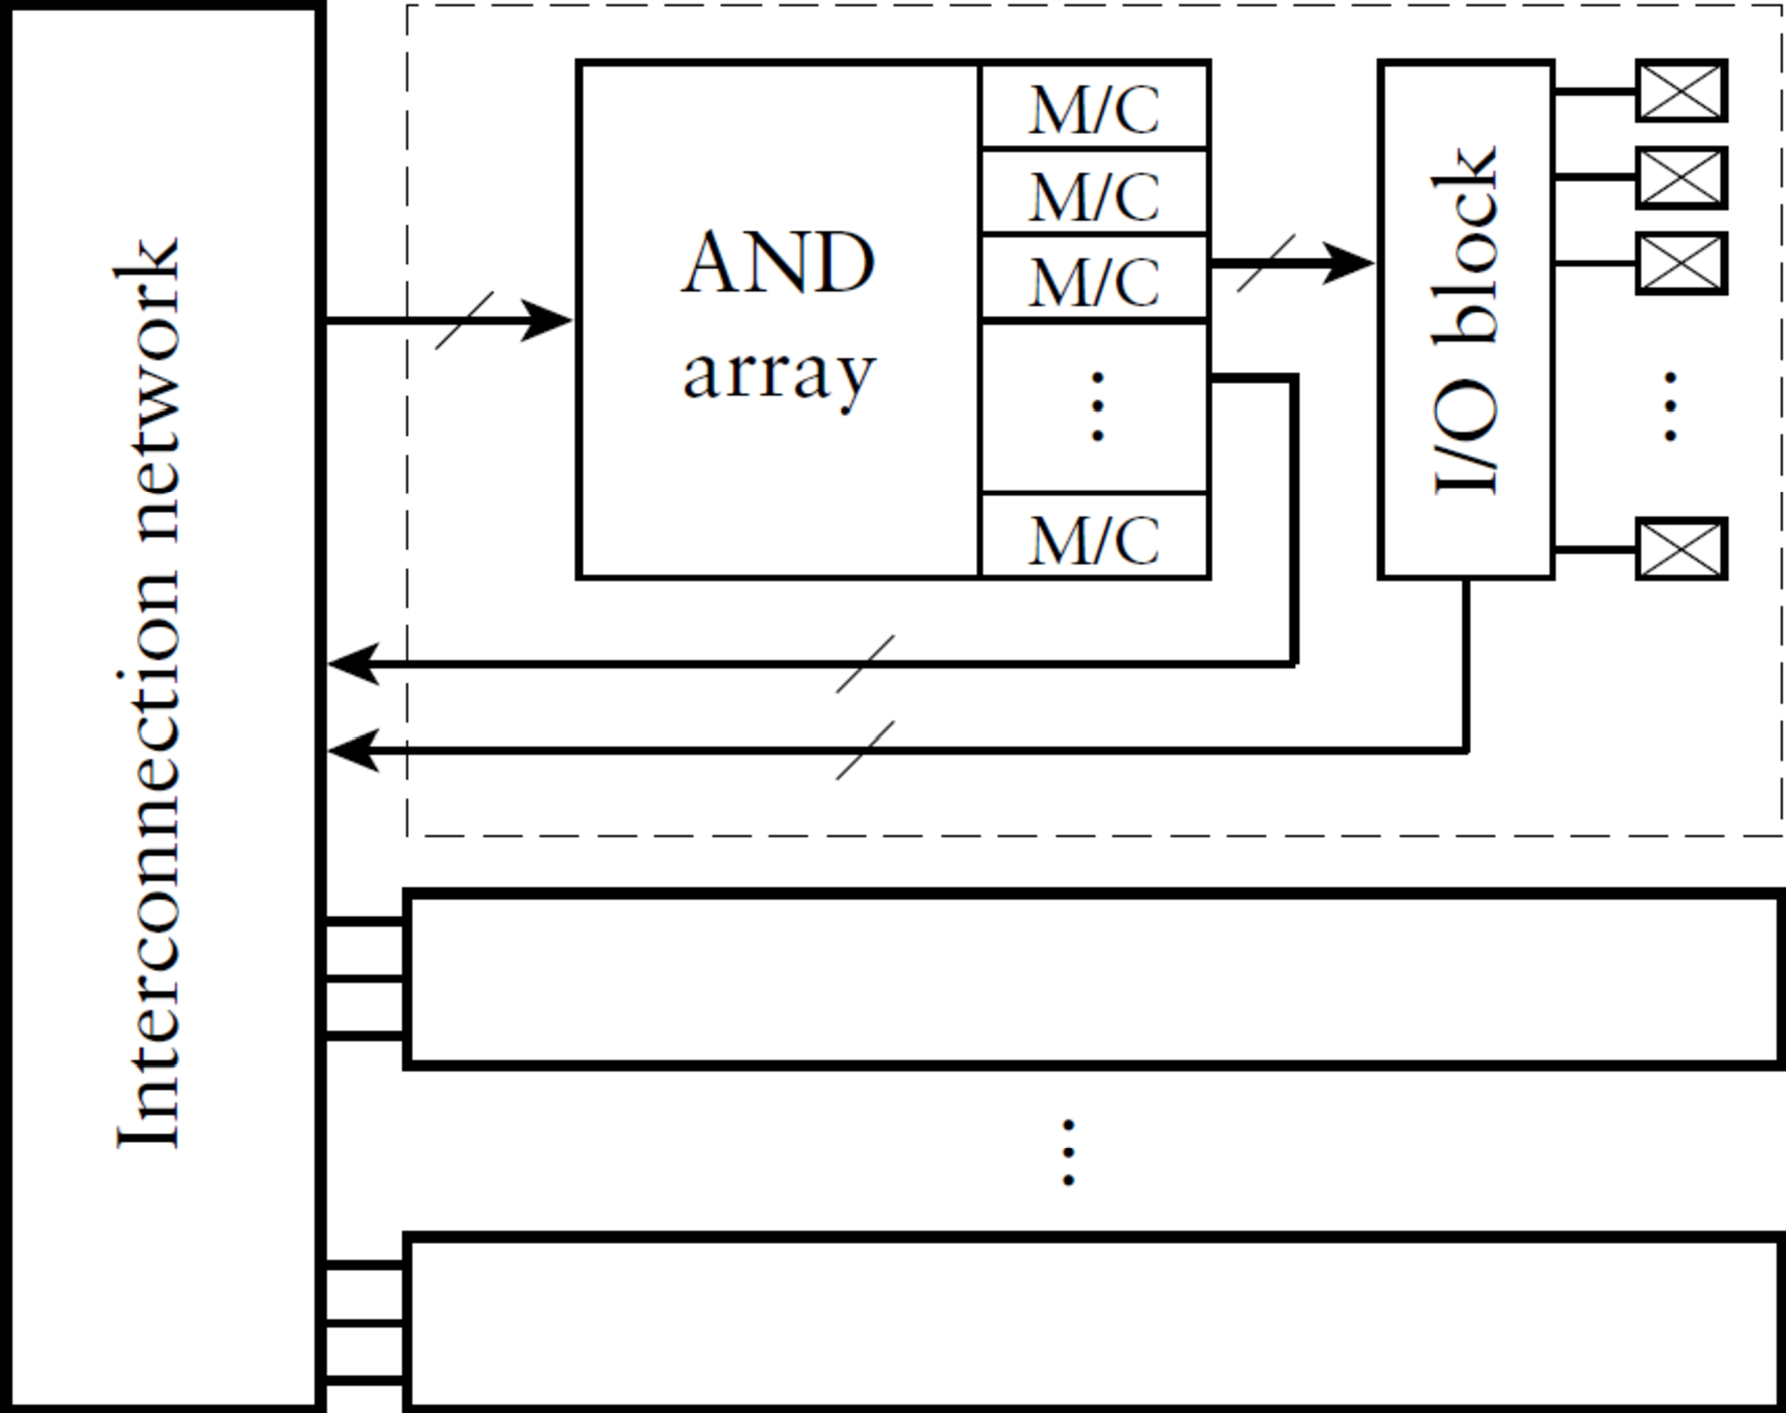
\includegraphics[width=0.5\textwidth]{fig/c1_introducao/model_cpld.pdf}
\caption{Representa\c{c}\~ao de dispositivos do tipo CPLD, extraido de \cite{Ashenden2008}.}
\label{fig:cpld}
\end{figure}

\paragraph{\textit{Complex Programmable Logic Device}}
Desenvolvida depois dos PALs, os CPLDs s\~ao dispositivos similares aos PALs, mas com suporte a um n\'umero maior de blocos l\'ogicos.
Eles podem ser definidos como um conjundo de PALs conectados por uma rede program\'avel de conex\~oes, como tenta esquematizar a figura \ref{fig:cpld}.
Sua arquitetura \'e baseada no mar de portas, como mostra a figura \ref{fig:cpld}.
Detalhes de implementa\c{c}\~ao variam de fabricante.

Al\'em de conter mais recursos que os PALs, os CPLDs s\~ao diferentes na forma de programa\c{c}\~ao.
Ao inv\'es de usar EEPROM, eles usam mem\'orias RAM n\~ao-vol\'ateis para armazenar a programa\c{c}\~ao quando o sistema \'e desligado e c\'elulas de mem\'oria SRAM para armazenar as informa\c{c}\~oes de conex\~oes e comportamento das c\'elulas l\'ogicas.
Quando o dispositivo \'e energizado, a programa\c{c}\~ao da mem\'oria RAM \'e passada para as c\'elulas SRAM, que permitem que o sistema funcione.
A mem\'oria n\~ao-vol\'atil tamb\'em possui pinos independentes acess\'i­veis externamente, o que permitem que ele seja programado mesmo depois de soldado ao produto final permitindo sua atualiza\c{c}\~ao.

A maior vantagem dos CPLDs com rela\c{c}\~ao a outros dispositivos \'e a sua n\~ao-volatilidade, tornando-o muito \'util como \textit{bootloaders} ou em aplica\c{c}\~oes que precisem rodar assim que o sistema \'e energizado.
O mais famoso destes dispositivos, conhecido por Max, \'e desenvolvido pela Altera.

\begin{figure}[h]
\centering
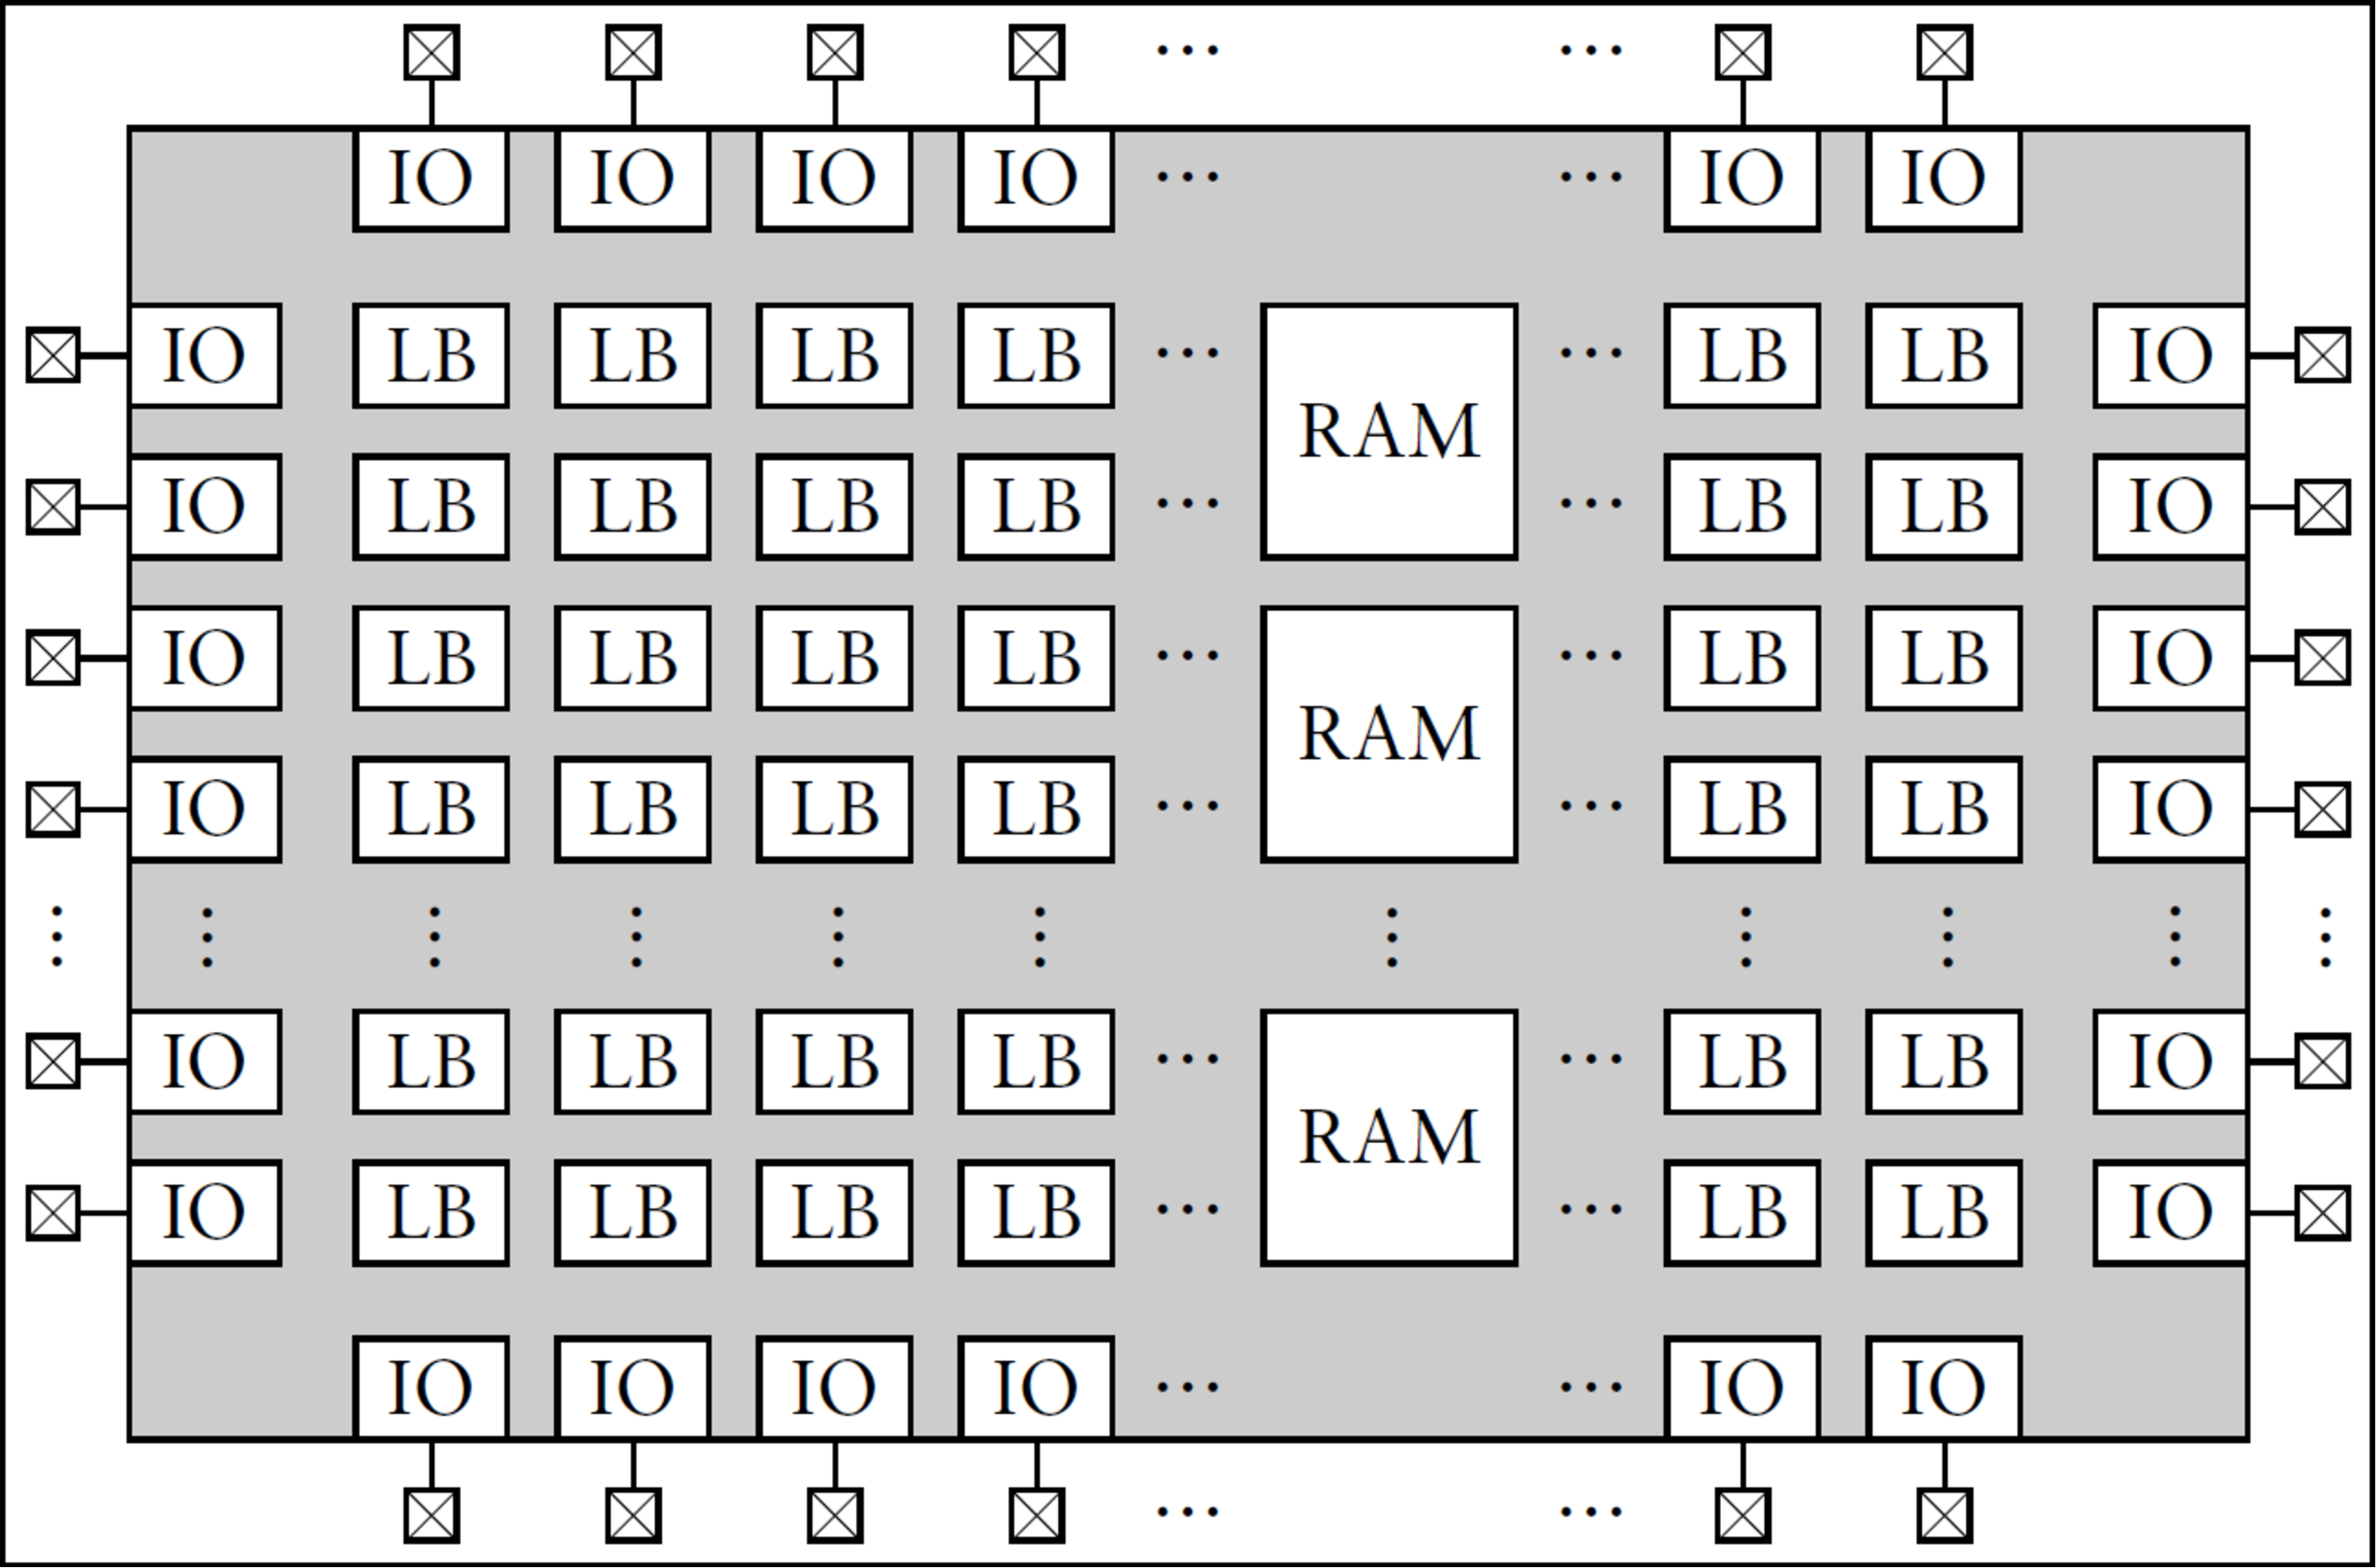
\includegraphics[width=0.65\textwidth]{fig/c1_introducao/model_fpga.pdf}
\caption{Representa\c{c}\~ao de dispositivos do tipo FPGA, extraido de \cite{Ashenden2008}.}
\label{fig:fpga}
\end{figure}

\paragraph{\textit{Field-Programmable Gate Array}}
Formado de c\'elulas program\'aveis consideravelmente menores que as dos CPLDs, que permitem uma maior integra\c{c}\~ao, existe o \textit{Field-Programmable Gate Array}.
Como se pode notar, este dispositivo possui dentre as suas caracter\'i­sticas principais a capacidade de ser programado e reprogramado em campo (\textit{field}), isto \'e, sem a necessidade de processos especiais.
Apesar disso, devido a complexidade dos circuitos internos destes dispositivos, simplificados na figura \ref{fig:fpga}, eles n\~ao foram feitos para serem programados manualmente, o que ainda era poss\'i­vel com os CPLDs, fazendo-se necess\'ario o uso de ferramentas de projeto auxiliado por computador (CAD) para, dado um c\'odigo em linguagem de descri\c{c}\~ao de \textit{hardware}, sintetizar, mapear, alocar e rotear o projeto automaticamente.

Desde a sua inven\c{c}\~ao, as FPGAs vem crescendo em capacidade e performance, tendo se tornado o principal componente de computa\c{c}\~ao reconfigur\'avel.
A maioria das suas implementa\c{c}\~oes se assemelha, em alto n\'i­vel, ao circuito apresentado na figura \ref{fig:fpga}.
Eles incluem blocos l\'ogicos que podem implementar tanto l\'ogicas combinacionais simples quanto fun\c{c}\~oes l\'ogicas sequenciais, blocos de entrada e sa\'i­da registrados ou n\~ao com possibilidade de funcionamento em diversos n\'i­veis l\'ogicos e condi\c{c}\~oes de temporiza\c{c}\~ao, c\'elulas de mem\'oria RAM embutidas e uma rede de conex\~oes program\'avel.
A raz\~ao para permitir que todas estas caracter\'i­sticas sejam programadas \'e permitir que os FPGAs sejam usados nos mais diversos tipos de sistemas, que usam diferentes padr\~oes de sinais entre \textit{chips}.
Detalhes de implementa\c{c}\~ao por\'em variam entre fabricantes e fam\'i­lias de dispositivos.
Apesar disso, em sua maioria, utilizam de mem\'orias RAM ass\'i­ncronas de 1 bit conhecidas como \textit{lookup tables} (LUTs), al\'em de \textit{flip-flops} e multiplexadores.
Algumas FPGAs tamb\'em incluem c\'elulas especializadas de processamento como multiplicadores e processadores gen\'ericos.

Existem dois tipos de FPGAs, um baseado em mem\'oria RAM e outro baseado em \textit{antifuses}.
Como foi falado na se\c{c}\~ao \ref{ss:computacao_reconfiguravel}, a mem\'oria RAM \'e vol\'atil, for\c{c}ando o sistema a ser programado toda vez que energizado.
Apesar disso, possui a vantagem de poder ter sua programa\c{c}\~ao modificada em campo.
O FPGA baseado em \textit{antifuses} s\'o pode ser programado uma vez, na f\'abrica.

\begin{table}[h]
\centering
\begin{tabular}{|c|c|c|c|}
\hline
 & PAL & CPLD & FPGA \\ \hline
Custo & \$2-\$15 & \$5-\$50 & \$10-\$300 \\ \hline
Blocos l\'ogicos & 8-10 & 32 - 128 & 100+ \\ \hline
Pinos de I/O & 20-24 & 44-160 & 84-256\\ \hline
Configura\c{c}\~ao & EEPROM & EEPROM & RAM ou OTP\\ \hline
Projeto & Equa\c{c}\~oes Booleanas & HDL ou esquem\'atico & HDL ou esquem\'atico\\ \hline
\end{tabular}
\caption{Tabela comparativa dos dipositivos reconfigur\'aveis dos tipos PAL, CPLD e FPGA.}
\label{tab:comparacao}
\end{table}

A tabela \ref{tab:comparacao} apresenta uma compara\c{c}\~ao ligeiramente grosseira entre os PALs, CPLDs e FPGAs.

\begin{figure}[h]
\centering
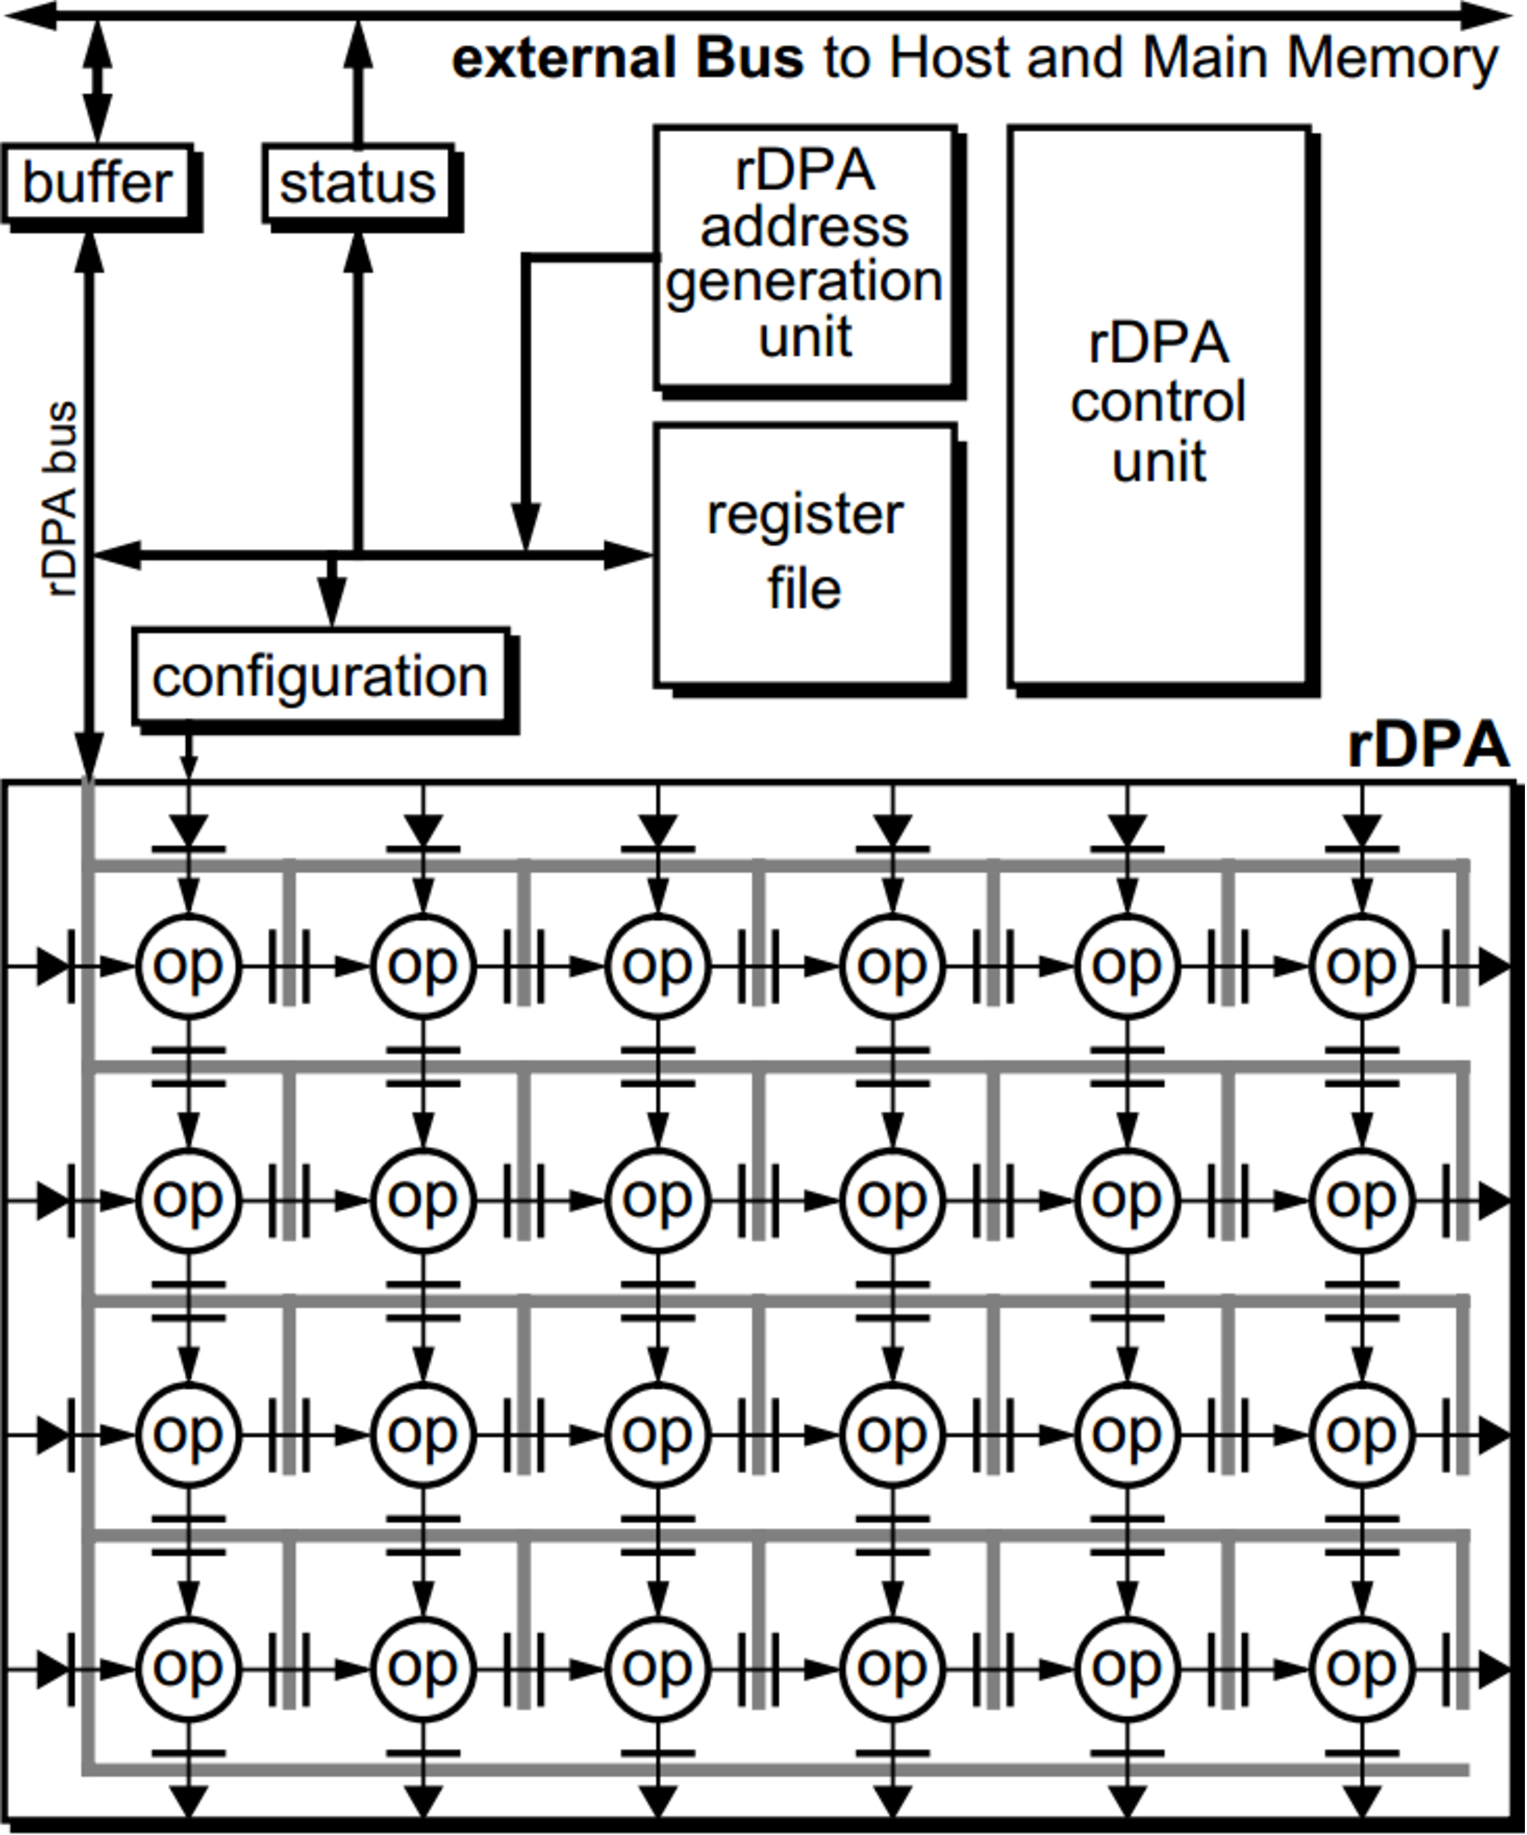
\includegraphics[width=0.5\textwidth]{fig/c1_introducao/model_rdpa.pdf}
\caption{Modelo de rDPA do tipo KressArray-I, extraido de \cite{Hartenstein1995}.}
\label{fig:kressarray}
\end{figure}

\paragraph{\textit{Reconfigurable Datapath Array}}
O \textit{Reconfigurable Datapath Array} \'e um tipo de sistema reconfigur\'avel com granularidade grossa, normalmente 32 bits \cite{Hartenstein2001}.
Apesar de relativamente mais novo que os dispositivos abaixo, ele \'e menos utilizado.
Seus blocos l\'ogicos, chamados de \textit{datapath processing units} (DPUs), s\~ao um pouco mais complexos que os dispositivos de granularidade fina de forma a conseguir tratar os dados maiores.
Eles possuem m\'ultiplas conex\~oes uni e birecionais entre seus vizinhos diretos, al\'em de trilhas verticais/horizontais completas ou segmentadas e um trilha principal mais externa que conecta todos os blocos, conforme mostra a figura \ref{fig:kressarray}.
As vantagens deste tipo de sistema reconfigur\'avel s\~ao um maior poder de processamento para uma mesma complexidade de roteamento em rela\c{c}\~ao aos sistemas de granularidade mais fina al\'em de um tempo de configura\c{c}\~ao reduzido.
Em todos os outros aspectos, ele \'e extremamente similar a FPGAs.
Sua desvantagem \'e o baixo controle dos bits individuais, uma vez que mesmo a descri\c{c}\~ao de \textit{hardware} indique o uso de apenas um bit, toda uma palavra \'e usada.

\subsubsection{Linguagens de Descri\c{c}\~ao de \textit{Hardware}}
Um dispositivo reconfigur\'avel precisa de informa\c{c}\~oes sobre o seu comportamento desejado para poder ser configurado.
O primeiro passo desse processo \'e a descri\c{c}\~ao do sistema por uma linguagem de programa\c{c}\~ao similar as usadas em computa\c{c}\~ao geral.
Dentre as linguagens mais comuns est\~ao Verilog, VHDL e SystemC.

Verilog e VHDL descrevem o sistema atrav\'es da abstra\c{c}\~ao em \textit{Register-Transfer Level} (RTL), ou seja, o comportamento dos circuitos digitais s\'i­ncronos \'e definido em termos do seu fluxo de dados e opera\c{c}\~oes realizadas.
SystemC por outro lado usa o \textit{Transaction-Level Modeling}, que descreve o comportamento do circuito atrav\'es de modelos de canais de comunica\c{c}\~oes.
Os m\'odulos funcionais ent\~ao realizam transa\c{c}\~oes de informa\c{c}\~oes entre si.

Al\'em das linguagem j\'a mencionadas, outra classe de linguagens de descri\c{c}\~ao de \text{hardware} \'e conhecida como \text{Analog Mixed-Signal} (AMS), sendo basicamente extens\~oes das linguagens j\'a mencionadas.
Estas extens\~oes acrescentam a linguagem a capacidade de trabalhar com sinais anal\'ogicos.
Tais linguagens tem sido bastante usadas em simula\c{c}\~oes, mas deixadas de lado na etapa de s\'i­ntese pela falta de ferramentas.

\todo{Comentar sobre a programação estrutural e comportamental.}

\paragraph{Verilog}
Verilog foi a primeira linguagem moderna de descri\c{c}\~ao de \textit{hardware}.
Ela foi desenvolvida com a inten\c{c}\~ao apenas de descrever e simular/validar circuitos digitais, mas nos anos seguintes a op\c{c}\~ao de s\'i­ntese foi acrescentada.
Padronizada pelo IEEE em 1995, o Verilog foi desenvolvido para ser similar a linguagem de programa\c{c}\~ao gen\'erica "C".

\todo{Comentar a possibilidade de programação estrutural e comportamental, bem como imbutir informações de simulação e timing no Verilog \cite{Thomas1996}.}

\paragraph{VHDL}
VHDL foi desenvolvida logo em seguida ao Verilog, em um projeto solicitado pelo Departamento de Defesa dos Estados Unidos, como uma forma de documentar o comportamento de ASICs.
Ela possui uma sintaxe similar a linguagem "Ada".
A linguagem logo foi padronizada pelo IEEE, em 1987.
Ela possui algumas diferen\c{c}as b\'asicas em rela\c{c}\~ao ao Verilog que n\~ao ser\~ao mencionados aqui.
A maior diferen\c{c}a pr\'atica por\'em \'e a presen\c{c}a de bibliotecas padronizadas pelo IEEE que disponibilizam funcionalidades muito \'uteis.

\todo{Comentar sobre a programação estrutural e comportamental e dar mais importancia as bibliotecas do VHDL.}

\paragraph{SystemC}
SystemC foi desenvolvida em meados dos anos 2000, aproximadamente 15 anos depois do Verilog e VHDL, com o intuido de aproximar as linguagens de descri\c{c}\~ao de \textit{hardware} \`as de programa\c{c}\~ao gen\'erica.
Ela \'e basicamente um conjunto de classes e macros para "C++" que disponibiliza uma interface de simula\c{c}\~ao dirigidas por eventos.
Essas ferramentas permitem que o projetista simule processos concorrentes, mas nos \'ultimos tempos tamb\'em foi adaptada para o desenvolvimento de sistemas reconfigur\'aveis.
Uma vez que n\~ao foi desenvolvida com o prop\'osito principal de descric\~ao de \text{hardware}, possui um chamado "\textit{overhead} sint\'atico" com rela\c{c}\~ao a Verilog e VHDL, onde mais texto tem que ser escrito para descrever um mesmo comportamento.

\subsection{Classes de Reconfigura\c{c}\~ao}
Com a chegada de CPLDs e FPGAs, requisitos cada vez mais complexos foram sendo introduzidos ao projeto de sistemas digitais.
Tais requisitos for\c{c}aram as ferramentas de s\'i­ntese a suportar diferentes classes de reconfigura\c{c}\~ao.
Note que reconfigura\c{c}\~ao diz respeito, como dito anteriormente, a modifica\c{c}\~ao do comportamento, ou configura\c{c}\~ao, de um dispositivo reconfigur\'avel.

\subsubsection{Reconfigura\c{c}\~ao Total}
A reconfigura\c{c}\~ao total, herdada da tecnologia tradicional, compreende a mudan\c{c}a do comportamento de todo o dispositivo reconfigur\'avel, sem exce\c{c}\~ao de blocos l\'ogicos.
Tal reconfigura\c{c}\~ao \'e bastante dispendiosa, visto que maior parte das alterações realizadas são incrementais e dizem respeito \`a apenas uma pequena parte do dispositivo.
Apesar disto, todos os FPGAs d\~ao suporte a este tipo de reconfigura\c{c}\~ao.

\subsubsection{Reconfigura\c{c}\~ao Parcial}
A reconfigura\c{c}\~ao parcial, ao contr\'ario da reconfigura\c{c}\~ao total, diz respeito \`a programa\c{c}\~ao de apenas parte de um dispositivo reconfigur\'avel \cite{Hauck2007}.
Para tal, faz-se necess\'ario a divis\~ao do dispositivo nas chamadas parti\c{c}\~oes, cada uma com sua configura\c{c}\~ao individual.
Desta forma, mudan\c{c}as feitas em uma parti\c{c}\~ao n\~ao afetam as outras, acelerando o processo de s\'i­ntese e programa\c{c}\~ao.
Outro processo que \'e acelerado \'e o de roteamento, uma vez que o particionamento introduz limita\c{c}\~oes no mapeamento das fun\c{c}\~oes.
Nem todos os FPGAs d\~ao suporte a este tipo de reconfigura\c{c}\~ao, que pode ser realizado tanto de forma dinâmica (\ref{sss:dinamica}) quando estática (\ref{sss:estatica}).

\subsubsection{Reconfigura\c{c}\~ao Est\'atica}
\label{sss:estatica}
O termo reconfigura\c{c}\~ao est\'atica se refere a programa\c{c}\~ao de um dispositivo reconfigur\'avel enquanto ele n\~ao estiver executando.
No caso em que alguma programa\c{c}\~ao j\'a tenha sido transferida para ele e ele a esteja executando, esta \'e parada para que o dispositivo seja configurado novamente.
Por ser mais f\'acil de ser implementada e n\~ao necessita de circuitos adicionais, todos os FPGAs d\~ao suporte a este tipo de reconfigura\c{c}\~ao.

\subsubsection{Reconfigura\c{c}\~ao Din\^amica}
\label{sss:dinamica}
A reconfigura\c{c}\~ao din\^amica acontece frente \`a necessidade de reprograma\c{c}\~ao parcial do dispositivo sem que ele pare de funcionar.
As funcionalidades modificadas s\~ao interrompidas e substituidas sem afetar o funcionamento do todo.
Normalmente este processo, quando n\~ao associado a autorreconfigura\c{c}\~ao, \'e realizado atrav\'es de um circuito externo à FPGA, tal como um controlador, um microcontrolador, ou mesmo um computador, como apresentado na figura \ref{fig:rexterna}.
Quase todos os FPGAs modernos d\~ao suporte a esta tecnologia.

\begin{figure}[htp]
\centering
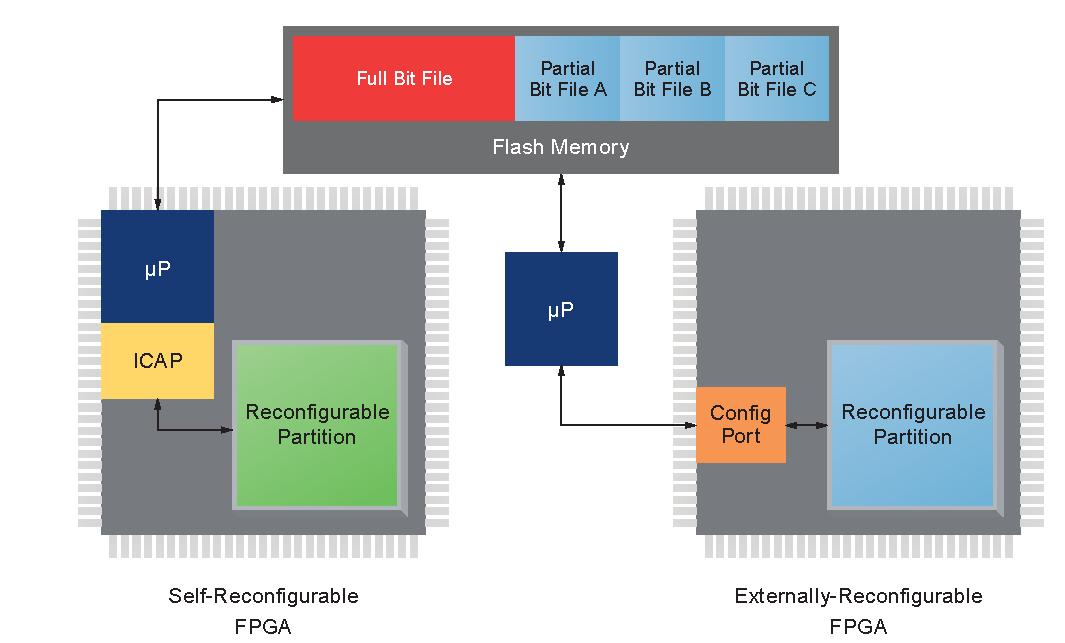
\includegraphics[width=0.8\textwidth]{fig/c1_introducao/reconf_externa.pdf}
\caption{Imagem ilustrativa para diferenciação entre autorreconfiguração e reconfiguração externa, extraido de \cite{wp374}.}
\label{fig:rexterna}
\end{figure}

É implicito o uso da reconfiguração parcial com a reconfiguração dinâmica, uma vez que faz pouco sentido reconfigurar todo o FPGA enquanto ela ainda está em execução.
Note que este tipo de reconfiguração em geral também necessita de uma parte permanentemente est\'atica, para interfacear com o circuito controlador.
Esta parti\c{c}\~ao est\'atica \'e respons\'avel pelo menos por controlar a comunica\c{c}\~ao com o circuito controlador.

Vale lembrar que a este tipo de reconfiguração, apesar de abrir muitas possibilidades, introduz uma necessidade de preocupação com \textit{overheads} de reconfiguração \cite{Hauck2007}.
Este \textit{overhead} é proporcional ao tamanho da partição que se deseja modificar e inversamente proporcional às velocidades das interfaces de reconfiguração.
Tal fator pode se tornar crucial na escolha entre o uso desta tecnologia ou alguma outra alternativa, possivelmente multiplexada.
Note que existem outros fatores que influenciam na opção por reconfiguração dinâmica, tais como preço, capacidade e potência, dentre outros, que não serão considerados aqui.

\subsubsection{Autorreconfigura\c{c}\~ao}
Modalidade de reconfigura\c{c}\~ao din\^amica parcial onde a reconfigura\c{c}\~ao do dispositivo \'e decidida por uma l\'ogica pertencente a ele mesmo.
Normalmente usa-se um microcontrolador ou uma m\'aquina de estados finitos para controlar a mudan\c{c}a de configura\c{c}\~oes.
Este tecnologia \'e nova e ainda representa uma forte \'area de pesquisa.
Por isso n\~ao s\~ao todos os FPGAs que d\~ao suporte a este tipo de reconfigura\c{c}\~ao.

Para que a autorreconfigura\c{c}\~ao aconte\c{c}a, os \textit{bitstreams}, resultado da sintetiza\c{c}\~ao, devem ser passados para uma mem\'oria acess\'i­vel ao FPGA durante a execu\c{c}\~ao do mesmo.
O circuito controlador identifica ent\~ao um padr\~ao que defina a necessidade de reconfigura\c{c}\~ao e transfere o \textit{bitstream} correspondente a esta nova necessidade para a parti\c{c}\~ao destino, que assim muda seu comportamento.
Note que para tal, as entradas e sa\'i­das das parti\c{c}\~oes tem que ser fixas, para que a mudan\c{c}a nas configura\c{c}\~oes das parti\c{c}\~oes n\~ao danifique o FPGA em si.

\subsection{Dispositivos e Ferramentas}
As duas maiores fabricantes de FPGAs s\~ao as empresas Altera e Xilinx.
A Xilinx foi a primeira fabricante de FPGAs do mundo e det\'em aproximadamente 51\% do mercado de FPGAs, enquanto a Altera, sua maior competitora, possui aproximadamente 34\% do mercado.
Ambas possuem uma ampla linha de FPGAs e CPLDs.
Eles ser\~ao descritos abaixo.

\subsubsection{Altera}
A Altera possui diversas linhas de FPGAs, dentre elas uma de baixo custo, chamada Cyclone, uma de m\'edio custo, chamada Aria, e uma de alto, chamada Stratix, CPLDs, chamada Max, e uma s\'erie de ASICs, chamada \textit{HardCopy}.
Todos os seus dispositivos s\~ao programados a partir de um programa chamado Quartus, hoje na sua segunda vers\~ao.
O Quartus possui ferramentas para a programa\c{c}\~ao do comportamento do sistema, simula\c{c}\~ao, s\'i­ntese, programa\c{c}\~ao do \textit{bitstream} do FPGA, constru\c{c}\~ao de \textit{System-on-Chips} (SoCs), IDE para programa\c{c}\~ao destes SoCs e ferramentas para a verifica\c{c}\~ao de projetos.
Apesar da sua variada linha de dispositivos, sintetizada na tabela \ref{tab:altera} e poderosa ferramenta de programa\c{c}\~ao, a Altera apresenta poucas s\'eries com possibilidade de reconfigura\c{c}\~ao parcial e autorreconfigura\c{c}\~ao.

\begin{table}[h]
\centering
\begin{tabular}{|c|l|p{6.5cm}|}
\hline
Tipo & Fam\'i­lia & Breve Descri\c{c}\~ao \\ \hline
CPLD & MAX\textsuperscript{\textregistered} II & Tecnologia com numerosos blocos similares aos PALs. \\ \hline
FPGA & Cyclone & Baixo custo, repleto de elementos de mem\'oria \\ \hline
FPGA & Arria\textsuperscript{\textregistered} & Série \textit{midrange}, com desempenho superior a Cyclone e inferior a Stratix. Pode ter \textit{transceivers}. \\ \hline
FPGA & Stratix\textsuperscript{\textregistered} & Alta performance, baixa pot\^encia. \\ \hline
FPGA & Stratix\textsuperscript{\textregistered} GX & S\'erie com \textit{transceivers} seriais e \textit{arrays} de alta performance escal\'aveis. \\ \hline
ASIC & HardCopy\textsuperscript{\textregistered} & S\'erie de ASICs estruturados de baixo custo e alta performance.\\ \hline
\end{tabular}
\caption{Fam\'i­lias de produtos da Altera, como apresentado em \cite{Woods2008}.}
\label{tab:altera}
\end{table}

\todo{Descrever melhor os produtos da Altera, atualizando tabela}

O sistema de desenvolvimento da Altera, chamado Quartus, dá suporte a todos os dispositivos da empresa a partir da instalação de pacotes com informações dos mesmos.
Apesar de muito robusto, este programa dá suporte a tecnologias mais atuais, como reconfiguração parcial ou dinâmica, através de extensões e componentes de propriedade intelectual (IP).
Estas tecnologias, pórem, só estão disponíveis para alguns dispositivos mais avançados e caros, tipicamente com \textit{transceivers}, do portfolio da companhia.

\subsubsection{Xilinx}
A Xilinx foi a respons\'avel pela inven\c{c}\~ao do FPGA.
Ela atualmente possui cinco fam\'i­lias de FPGAs, as quais est\~ao apresentadas, conforme mostrado em \cite{Woods2008}, na tabela \ref{tab:xilinx}.
Note que alguns dispositivos mais novos est\~ao ausentes desta tabela.
A Xilinx disponibiliza, como a Altera, ferramentas integradas de desenvolvimento de \textit{hardware}, chamadas ISE e Vivado.
O motivo da presen\c{c}a de duas ferramentas diferentes para uma mesma empresa \'e a recente aquisi\c{c}\~ao da ferramenta Vivado, mais eficiente que a ISE.
Al\'em das funcionalidades oferecidas pela ferramenta da Altera, as ferramentas da Xilinx possuem ainda a capacidade de utilizar FPGAs como aceleradoras com uso do MatLab.
Esta fun\c{c}\~ao permite que o projeto seja sintetizado e passado para uma FPGA real, mas que as entradas e sa\'i­das sejam controladas em um ambiente de simula\c{c}\~ao do MatLab chamado de Simulink.

\begin{table}[h]
\centering
\begin{tabular}{|c|l|p{6.5cm}|}
\hline
Tipo & Fam\'i­lia & Breve Descri\c{c}\~ao \\ \hline
CPLD & XC9500XL & Tecnologia CPLD antiga. \\ \hline
CPLD & CoolRunner & CPLD de alta performance e baixo consumo. \\ \hline
FPGA & Virtex/E/EM & Fam\'i­lia principal da Xilinx, FPGAs de alta performance. \\ \hline
FPGA & Spartan & FPGA de baixo custo e alto volume de vendas. \\ \hline
\end{tabular}
\caption{Fam\'i­lias de produtos da Xilinx, como apresentado em \cite{Woods2008}.}
\label{tab:xilinx}
\end{table}

\todo{Descrever melhor os produtos da Xilnx, atualizando tabela}
\todo{Falar do ISE e do Vivado}

\section{Projeto}
\label{sec:projeto}
\todo{Descrever objetivos do projeto}

%\section{Metodologia}
%\subsection{Fluxo de Projeto}
%\subsubsection{Particionamento}
%\subsubsection{Aloca\c{c}\~ao}
%\subsubsection{S\'i­ntese}
%\label{sss:sintese}

\ifx\compilewholereport\undefined
	\bibliographystyle{authordate1} 
	%\bibliography{bibliografia}
	\newsavebox\mytempbib\savebox\mytempbib{\parbox{\textwidth}{\bibliography{bibliografia}}}

	\end{document}
\fi